% Seminarul 7: Ipoteza piețelor eficiente, mersul aleator și testele VR
% Statistica piețelor financiare -- Program de licență, Academia de Studii Economice din București
% GENERAT de latex/build_seminar7.py -- modificați generatorul, nu acest fișier.
% Implicit versiunea pentru studenți; versiunea profesorului este wrapper-ul *_solutions.tex.
\makeatletter\@ifundefined{ifsolutions}{\expandafter\newif\csname ifsolutions\endcsname}{}\makeatother

\newcommand{\coursename}{Statistica piețelor financiare}
\def\sfmlang{ro}
% Preambul comun SFM -- Statistica piețelor financiare / Statistics of Financial Markets (Beamer, 16:9)
% Același design ca MFM. Înainte de % Preambul comun SFM -- Statistica piețelor financiare / Statistics of Financial Markets (Beamer, 16:9)
% Același design ca MFM. Înainte de % Preambul comun SFM -- Statistica piețelor financiare / Statistics of Financial Markets (Beamer, 16:9)
% Același design ca MFM. Înainte de \input{../../latex/preamble} se definește
%   \newcommand{\coursename}{Statistics of Financial Markets}      (EN)
%   \newcommand{\coursename}{Statistica piețelor financiare}       (RO)  și  \def\sfmlang{ro}
% Fișierele .tex se află în EN/Courses, EN/Seminars, RO/Cursuri, RO/Seminarii (două niveluri sub rădăcină).
% Deck-urile sînt generate de latex/build_chapterN.py / build_seminarN.py (vezi latex/sfm_build.py).

\documentclass[9pt, aspectratio=169, t]{beamer}
\providecommand{\coursename}{Statistics of Financial Markets}

% Ensure content fits on slides
\setbeamersize{text margin left=8mm, text margin right=8mm}

%=============================================================================
% THEME AND STYLE CONFIGURATION
%=============================================================================
\usetheme{default}
% Using default theme for clean header/footer control

% Color Palette (matching Redispatch PDF)
\definecolor{MainBlue}{RGB}{26, 58, 110}
\definecolor{AccentBlue}{RGB}{26, 58, 110}
\definecolor{IDAred}{RGB}{205, 0, 0}
\definecolor{DarkGray}{RGB}{51, 51, 51}
\definecolor{MediumGray}{RGB}{128, 128, 128}
\definecolor{LightGray}{RGB}{248, 248, 248}
\definecolor{VeryLightGray}{RGB}{235, 235, 235}
\definecolor{KeynoteGray}{RGB}{218, 218, 218}
\definecolor{SectionGray}{RGB}{120, 120, 120}
\definecolor{FooterGray}{RGB}{100, 100, 100}
\definecolor{Crimson}{RGB}{220, 53, 69}
\definecolor{Forest}{RGB}{46, 125, 50}
\definecolor{Amber}{RGB}{181, 133, 63}
\definecolor{Orange}{RGB}{230, 126, 34}
\definecolor{Purple}{RGB}{142, 68, 173}

% Gradient background (exact Keynote 315° gradient: white to RGB 218,218,218)
\setbeamertemplate{background}{%
    \begin{tikzpicture}[remember picture, overlay]
        \shade[shading=axis, shading angle=315,
        top color=white, bottom color=KeynoteGray]
        (current page.south west) rectangle (current page.north east);
    \end{tikzpicture}%
}
% Fallback solid color for compatibility
\setbeamercolor{background canvas}{bg=}

\setbeamercolor{palette primary}{bg=MainBlue, fg=white}
\setbeamercolor{palette secondary}{bg=MainBlue!85, fg=white}
\setbeamercolor{palette tertiary}{bg=MainBlue!70, fg=white}
\setbeamercolor{structure}{fg=MainBlue}
\setbeamercolor{title}{fg=IDAred}
\setbeamercolor{frametitle}{fg=IDAred, bg=}
\setbeamercolor{block title}{bg=MainBlue, fg=white}
\setbeamercolor{block body}{bg=VeryLightGray, fg=DarkGray}
\setbeamercolor{block title alerted}{bg=Crimson, fg=white}
\setbeamercolor{block body alerted}{bg=Crimson!8, fg=DarkGray}
\setbeamercolor{block title example}{bg=Forest, fg=white}
\setbeamercolor{block body example}{bg=Forest!8, fg=DarkGray}
\setbeamercolor{item}{fg=MainBlue}

% Footer colors (override Madrid theme blue)
\setbeamercolor{author in head/foot}{fg=FooterGray, bg=}
\setbeamercolor{title in head/foot}{fg=FooterGray, bg=}
\setbeamercolor{date in head/foot}{fg=FooterGray, bg=}
\setbeamercolor{section in head/foot}{fg=FooterGray, bg=}
\setbeamercolor{subsection in head/foot}{fg=FooterGray, bg=}

% Bullet styles (apply everywhere including blocks)
\setbeamertemplate{itemize item}{\color{MainBlue}$\boxdot$}
\setbeamertemplate{itemize subitem}{\color{MainBlue}$\blacktriangleright$}
\setbeamertemplate{itemize subsubitem}{\color{MainBlue}\tiny$\bullet$}
\setbeamertemplate{itemize/enumerate body begin}{\normalsize}
\setbeamertemplate{itemize/enumerate subbody begin}{\normalsize}

% Item spacing - compact style
\setlength{\leftmargini}{10pt}       % Level 1: minimal indent
\setlength{\leftmarginii}{10pt}      % Level 2: minimal additional indent
% Compact list spacing (zero extra space before/after lists in blocks)
\makeatletter
\def\@listi{\leftmargin\leftmargini \topsep 0pt \parsep 0pt \itemsep 0pt}
\def\@listii{\leftmargin\leftmarginii \topsep 0pt \parsep 0pt \itemsep 0pt}
\makeatother

\setbeamertemplate{navigation symbols}{}

%=============================================================================
% CUSTOM HEADLINE
%=============================================================================
\setbeamertemplate{headline}{%
    \vskip10pt%
    \hbox to \paperwidth{%
        \hskip0.5cm%
        {\small\color{FooterGray}\renewcommand{\hyperlink}[2]{##2}\insertsectionhead}%
        \hfill%
        \textcolor{FooterGray}{\small\insertframenumber}%
        \hskip0.5cm%
    }%
    \vskip4pt%
    {\color{FooterGray}\hrule height 0.4pt}%
}

%=============================================================================
% CUSTOM FOOTER
%=============================================================================
\usepackage{fontawesome5}

\setbeamertemplate{footline}{%
    {\color{FooterGray}\hrule height 0.4pt}%
    \vskip4pt%
    \hbox to \paperwidth{%
        \hskip0.5cm%
        \textcolor{FooterGray}{\small\coursename}%
        \hfill%
        \raisebox{-0.1em}{%
            \begin{tikzpicture}[x=0.08em, y=0.08em, line width=0.4pt]
                \draw[FooterGray] (0,3) -- (1,4) -- (2,3.5) -- (3,5) -- (4,4) -- (5,6) -- (6,5.5) -- (7,4) -- (8,5) -- (9,7) -- (10,6) -- (11,5) -- (12,6.5) -- (13,8) -- (14,7) -- (15,6) -- (16,7.5) -- (17,9) -- (18,8) -- (19,7) -- (20,8.5) -- (21,10) -- (22,9) -- (23,8) -- (24,9.5);
            \end{tikzpicture}%
        }%
        \hskip0.5cm%
    }%
    \vskip6pt%
}

%=============================================================================
% PACKAGES
%=============================================================================
\usepackage[utf8]{inputenc}
\DeclareUnicodeCharacter{03B1}{\ensuremath{\alpha}}
\usepackage[T1]{fontenc}
\usepackage{amsmath, amssymb, amsthm}
\usepackage{mathtools}
\usepackage{bm}
\usepackage{tikz}
\usetikzlibrary{arrows.meta, positioning, shapes, calc, decorations.pathreplacing, shadings}
\usepackage{booktabs}
\usepackage{multirow}
\usepackage{array}
\usepackage{graphicx}
\usepackage{hyperref}
\usepackage{colortbl}
\usepackage{listings}
\lstset{language=Python, basicstyle=\ttfamily\scriptsize, keywordstyle=\color{MainBlue}\bfseries,
  commentstyle=\color{Forest}, stringstyle=\color{Crimson}, breaklines=true,
  frame=none, backgroundcolor=\color{VeryLightGray}, xleftmargin=2mm}
\hypersetup{colorlinks=true, linkcolor=MainBlue, urlcolor=MainBlue}
\graphicspath{{../../logos/}{../../charts/}{../../photos/}}
\usepackage{xcolor}
\hfuzz=2pt  % Suppress tiny overfull warnings (<2pt)
\vfuzz=2pt  % Suppress tiny vertical overfull warnings (<2pt)

%=============================================================================
% QUANTLET COMMANDS
%   \quantlet{<displayed name>}{<url>}       (generic, compatible with the older SFM decks)
%   \sfmquantlet{Ch_05}{SFM_ch5_garch}       -> https://github.com/danpele/SFM/tree/main/Quantlets/Ch_05/SFM_ch5_garch
%   \qlurl{<folder>} is defined per chapter by the generator (Quantlets/Ch_NN/<folder>)
%=============================================================================
\newcommand{\sfmrepo}{https://github.com/danpele/SFM}
\newcommand{\sfmqlbase}{https://github.com/danpele/SFM/tree/main/Quantlets}
\newcommand{\quantlet}[2]{%
    \hfill\href{#2}{%
        \raisebox{-0.15em}{
\includegraphics[height=0.7em]{ql_logo.png}}%
        \textcolor{MainBlue}{\tiny\ #1}%
    }%
}
\newcommand{\sfmquantlet}[2]{\quantlet{\detokenize{#2}}{\sfmqlbase/#1/#2}}

%=============================================================================
% NOTEBOOKS (Google Colab)
%   \colaburl{notebooks/EN/chapter5_seminar_notebook.ipynb} -> the Colab link of a file in the SFM repo
%   \nb: the chapter notebook (each seminar deck redefines it with \renewcommand)
%=============================================================================
\newcommand{\colaburl}[1]{https://colab.research.google.com/github/danpele/SFM/blob/main/#1}
\newcommand{\nb}{https://colab.research.google.com/github/danpele/SFM/tree/main/notebooks/EN}
\newcommand{\nbname}{notebooks/EN}

%=============================================================================
% SLIDE HELPERS (used by the generators; the same as in MFM)
%=============================================================================
% local font size for list bodies (the preamble forces \normalsize)
\newcommand{\itemsize}[1]{\setbeamertemplate{itemize/enumerate body begin}{#1}\setbeamertemplate{itemize/enumerate subbody begin}{#1}}
\newcommand{\intitle}[1]{{\hypersetup{urlcolor=white}#1}}   % white links inside coloured title bars
\newcommand{\imgcap}[1]{{\scriptsize #1}\\[0.5mm]}          % caption under a photo
\newcommand{\imgcredit}[2]{{\tiny\color{FooterGray}\href{#1}{#2}}}   % image credit: source URL, author/licence
\newcommand{\aiprompt}[1]{{\ttfamily\color{MainBlue}#1}}     % a prompt to an AI assistant

%=============================================================================
% SEMINARS: student version by default; the instructor wrapper *_solutions.tex sets \solutionstrue
%=============================================================================
\makeatletter\@ifundefined{ifsolutions}{\expandafter\newif\csname ifsolutions\endcsname}{}\makeatother
\newcommand{\solonly}[1]{\ifsolutions #1\fi}
\newcommand{\propsub}{\ifsolutions\else\framesubtitle{\ifdefined\sfmlang Rezolvarea se discută la seminar\else Solution discussed in class\fi}\fi}

%=============================================================================
% APPENDIX AND CHAPTER LINKS (latex/appendix_links.py writes the calls; it also re-declares these
% macros before \begin{document}, so the decks compile with or without this preamble block)
%=============================================================================
\providecommand{\sfmapplink}[3]{\hypertarget{#2}{}\hyperlink{#1}{\beamergotobutton{#3}}}
\providecommand{\sfmappback}[2]{\begin{tikzpicture}[remember picture,overlay]\node[anchor=south east] at ([xshift=-3mm,yshift=7mm]current page.south east){\hyperlink{#1}{\beamerreturnbutton{#2}}};\end{tikzpicture}}
\providecommand{\sfmchlink}[2]{\href{#1}{#2}}
\providecommand{\sfmchlinkt}[2]{\href{#1}{\usebeamercolor[fg]{frametitle}#2}}

%=============================================================================
% QUANTINAR COMMAND: link către un curs Quantinar (subiecte avansate)
%=============================================================================
\newcommand{\quantinar}[2]{%
    \href{#2}{%
        \raisebox{-0.15em}{
\includegraphics[height=0.8em]{qr_logo.png}}%
        \textcolor{MainBlue}{\scriptsize\ #1}%
    }%
}

%=============================================================================
% CUSTOM TITLE PAGE
%=============================================================================
\defbeamertemplate*{title page}{hybrid}[1][]
{
    \vspace{0.2cm}
    % Logos row - top header (with clickable links)
    \begin{center}
        \href{https://www.ase.ro}{
\includegraphics[height=1.0cm]{ase_logo.png}}\hspace{0.3cm}%
        \href{https://theida.net}{
\includegraphics[height=1.0cm]{ida_logo.png}}\hspace{0.3cm}%
        \href{https://blockchain-research-center.com}{
\includegraphics[height=1.0cm]{brc_logo.png}}\hspace{0.3cm}%
        \href{https://www.ai4efin.ase.ro}{
\includegraphics[height=1.0cm]{ai4efin_logo.png}}\hspace{0.3cm}%
        \href{https://ipe.ro/new}{
\includegraphics[height=1.0cm]{acad_logo.png}}\hspace{0.3cm}%
        \href{https://www.digital-finance-msca.com}{
\includegraphics[height=1.0cm]{msca_logo.png}}%
    \end{center}

    \vspace{0.6cm}

    % Main title with Q logos on sides (with clickable links)
    \begin{center}
        \begin{minipage}{0.1\textwidth}
            \centering
            \href{https://quantlet.com}{
\includegraphics[height=1.1cm]{ql_logo.png}}
        \end{minipage}%
        \begin{minipage}{0.78\textwidth}
            \centering
            {\LARGE\bfseries\usebeamercolor[fg]{title}\inserttitle}

            \vspace{0.3cm}

            {\usebeamerfont{subtitle}\usebeamercolor[fg]{title}\insertsubtitle}
        \end{minipage}%
        \begin{minipage}{0.1\textwidth}
            \centering
            \href{https://quantinar.com}{
\includegraphics[height=1.1cm]{qr_logo.png}}
        \end{minipage}
    \end{center}

    \vspace{0.6cm}

    % Authors (left aligned)
    \hspace{0.5cm}{\usebeamerfont{author}\insertauthor}

    \vspace{0.3cm}

    % Institute/Affiliations (left aligned)
    \hspace{0.5cm}\begin{minipage}[t]{0.9\textwidth}
        \raggedright\small\insertinstitute
    \end{minipage}
}

%=============================================================================
% THEOREM ENVIRONMENTS
%=============================================================================
\theoremstyle{definition}
\setbeamertemplate{theorems}[numbered]
\ifdefined\sfmlang
\newtheorem{defn}{Definiție}
\newtheorem{thm}{Teoremă}
\newtheorem{prop}{Propoziție}
\newtheorem{rmk}{Observație}
\else
\newtheorem{defn}{Definition}
\newtheorem{thm}{Theorem}
\newtheorem{prop}{Proposition}
\newtheorem{rmk}{Remark}
\fi

%=============================================================================
% CENTRED MINIPAGE (no extra vertical space)
%=============================================================================
\newenvironment{cminipage}[1]{%
    \par\noindent\hfill\begin{minipage}{#1}\ignorespaces
}{%
    \end{minipage}\hfill\null\par
}

%=============================================================================
% CUSTOM COMMANDS
%=============================================================================
\newcommand{\E}{\mathbb{E}}
\newcommand{\Var}{\text{Var}}
\newcommand{\Cov}{\text{Cov}}
\newcommand{\Corr}{\text{Corr}}
\newcommand{\R}{\mathbb{R}}
\newcommand{\N}{\mathbb{N}}
\newcommand{\Z}{\mathbb{Z}}
\newcommand{\B}{\mathbf{B}}
\newcommand{\imark}{\textcolor{MainBlue}{\textbullet}}
\newcommand{\RMSE}{\text{RMSE}}
\newcommand{\MAE}{\text{MAE}}
\newcommand{\MAPE}{\text{MAPE}}

 se definește
%   \newcommand{\coursename}{Statistics of Financial Markets}      (EN)
%   \newcommand{\coursename}{Statistica piețelor financiare}       (RO)  și  \def\sfmlang{ro}
% Fișierele .tex se află în EN/Courses, EN/Seminars, RO/Cursuri, RO/Seminarii (două niveluri sub rădăcină).
% Deck-urile sînt generate de latex/build_chapterN.py / build_seminarN.py (vezi latex/sfm_build.py).

\documentclass[9pt, aspectratio=169, t]{beamer}
\providecommand{\coursename}{Statistics of Financial Markets}

% Ensure content fits on slides
\setbeamersize{text margin left=8mm, text margin right=8mm}

%=============================================================================
% THEME AND STYLE CONFIGURATION
%=============================================================================
\usetheme{default}
% Using default theme for clean header/footer control

% Color Palette (matching Redispatch PDF)
\definecolor{MainBlue}{RGB}{26, 58, 110}
\definecolor{AccentBlue}{RGB}{26, 58, 110}
\definecolor{IDAred}{RGB}{205, 0, 0}
\definecolor{DarkGray}{RGB}{51, 51, 51}
\definecolor{MediumGray}{RGB}{128, 128, 128}
\definecolor{LightGray}{RGB}{248, 248, 248}
\definecolor{VeryLightGray}{RGB}{235, 235, 235}
\definecolor{KeynoteGray}{RGB}{218, 218, 218}
\definecolor{SectionGray}{RGB}{120, 120, 120}
\definecolor{FooterGray}{RGB}{100, 100, 100}
\definecolor{Crimson}{RGB}{220, 53, 69}
\definecolor{Forest}{RGB}{46, 125, 50}
\definecolor{Amber}{RGB}{181, 133, 63}
\definecolor{Orange}{RGB}{230, 126, 34}
\definecolor{Purple}{RGB}{142, 68, 173}

% Gradient background (exact Keynote 315° gradient: white to RGB 218,218,218)
\setbeamertemplate{background}{%
    \begin{tikzpicture}[remember picture, overlay]
        \shade[shading=axis, shading angle=315,
        top color=white, bottom color=KeynoteGray]
        (current page.south west) rectangle (current page.north east);
    \end{tikzpicture}%
}
% Fallback solid color for compatibility
\setbeamercolor{background canvas}{bg=}

\setbeamercolor{palette primary}{bg=MainBlue, fg=white}
\setbeamercolor{palette secondary}{bg=MainBlue!85, fg=white}
\setbeamercolor{palette tertiary}{bg=MainBlue!70, fg=white}
\setbeamercolor{structure}{fg=MainBlue}
\setbeamercolor{title}{fg=IDAred}
\setbeamercolor{frametitle}{fg=IDAred, bg=}
\setbeamercolor{block title}{bg=MainBlue, fg=white}
\setbeamercolor{block body}{bg=VeryLightGray, fg=DarkGray}
\setbeamercolor{block title alerted}{bg=Crimson, fg=white}
\setbeamercolor{block body alerted}{bg=Crimson!8, fg=DarkGray}
\setbeamercolor{block title example}{bg=Forest, fg=white}
\setbeamercolor{block body example}{bg=Forest!8, fg=DarkGray}
\setbeamercolor{item}{fg=MainBlue}

% Footer colors (override Madrid theme blue)
\setbeamercolor{author in head/foot}{fg=FooterGray, bg=}
\setbeamercolor{title in head/foot}{fg=FooterGray, bg=}
\setbeamercolor{date in head/foot}{fg=FooterGray, bg=}
\setbeamercolor{section in head/foot}{fg=FooterGray, bg=}
\setbeamercolor{subsection in head/foot}{fg=FooterGray, bg=}

% Bullet styles (apply everywhere including blocks)
\setbeamertemplate{itemize item}{\color{MainBlue}$\boxdot$}
\setbeamertemplate{itemize subitem}{\color{MainBlue}$\blacktriangleright$}
\setbeamertemplate{itemize subsubitem}{\color{MainBlue}\tiny$\bullet$}
\setbeamertemplate{itemize/enumerate body begin}{\normalsize}
\setbeamertemplate{itemize/enumerate subbody begin}{\normalsize}

% Item spacing - compact style
\setlength{\leftmargini}{10pt}       % Level 1: minimal indent
\setlength{\leftmarginii}{10pt}      % Level 2: minimal additional indent
% Compact list spacing (zero extra space before/after lists in blocks)
\makeatletter
\def\@listi{\leftmargin\leftmargini \topsep 0pt \parsep 0pt \itemsep 0pt}
\def\@listii{\leftmargin\leftmarginii \topsep 0pt \parsep 0pt \itemsep 0pt}
\makeatother

\setbeamertemplate{navigation symbols}{}

%=============================================================================
% CUSTOM HEADLINE
%=============================================================================
\setbeamertemplate{headline}{%
    \vskip10pt%
    \hbox to \paperwidth{%
        \hskip0.5cm%
        {\small\color{FooterGray}\renewcommand{\hyperlink}[2]{##2}\insertsectionhead}%
        \hfill%
        \textcolor{FooterGray}{\small\insertframenumber}%
        \hskip0.5cm%
    }%
    \vskip4pt%
    {\color{FooterGray}\hrule height 0.4pt}%
}

%=============================================================================
% CUSTOM FOOTER
%=============================================================================
\usepackage{fontawesome5}

\setbeamertemplate{footline}{%
    {\color{FooterGray}\hrule height 0.4pt}%
    \vskip4pt%
    \hbox to \paperwidth{%
        \hskip0.5cm%
        \textcolor{FooterGray}{\small\coursename}%
        \hfill%
        \raisebox{-0.1em}{%
            \begin{tikzpicture}[x=0.08em, y=0.08em, line width=0.4pt]
                \draw[FooterGray] (0,3) -- (1,4) -- (2,3.5) -- (3,5) -- (4,4) -- (5,6) -- (6,5.5) -- (7,4) -- (8,5) -- (9,7) -- (10,6) -- (11,5) -- (12,6.5) -- (13,8) -- (14,7) -- (15,6) -- (16,7.5) -- (17,9) -- (18,8) -- (19,7) -- (20,8.5) -- (21,10) -- (22,9) -- (23,8) -- (24,9.5);
            \end{tikzpicture}%
        }%
        \hskip0.5cm%
    }%
    \vskip6pt%
}

%=============================================================================
% PACKAGES
%=============================================================================
\usepackage[utf8]{inputenc}
\DeclareUnicodeCharacter{03B1}{\ensuremath{\alpha}}
\usepackage[T1]{fontenc}
\usepackage{amsmath, amssymb, amsthm}
\usepackage{mathtools}
\usepackage{bm}
\usepackage{tikz}
\usetikzlibrary{arrows.meta, positioning, shapes, calc, decorations.pathreplacing, shadings}
\usepackage{booktabs}
\usepackage{multirow}
\usepackage{array}
\usepackage{graphicx}
\usepackage{hyperref}
\usepackage{colortbl}
\usepackage{listings}
\lstset{language=Python, basicstyle=\ttfamily\scriptsize, keywordstyle=\color{MainBlue}\bfseries,
  commentstyle=\color{Forest}, stringstyle=\color{Crimson}, breaklines=true,
  frame=none, backgroundcolor=\color{VeryLightGray}, xleftmargin=2mm}
\hypersetup{colorlinks=true, linkcolor=MainBlue, urlcolor=MainBlue}
\graphicspath{{../../logos/}{../../charts/}{../../photos/}}
\usepackage{xcolor}
\hfuzz=2pt  % Suppress tiny overfull warnings (<2pt)
\vfuzz=2pt  % Suppress tiny vertical overfull warnings (<2pt)

%=============================================================================
% QUANTLET COMMANDS
%   \quantlet{<displayed name>}{<url>}       (generic, compatible with the older SFM decks)
%   \sfmquantlet{Ch_05}{SFM_ch5_garch}       -> https://github.com/danpele/SFM/tree/main/Quantlets/Ch_05/SFM_ch5_garch
%   \qlurl{<folder>} is defined per chapter by the generator (Quantlets/Ch_NN/<folder>)
%=============================================================================
\newcommand{\sfmrepo}{https://github.com/danpele/SFM}
\newcommand{\sfmqlbase}{https://github.com/danpele/SFM/tree/main/Quantlets}
\newcommand{\quantlet}[2]{%
    \hfill\href{#2}{%
        \raisebox{-0.15em}{
\includegraphics[height=0.7em]{ql_logo.png}}%
        \textcolor{MainBlue}{\tiny\ #1}%
    }%
}
\newcommand{\sfmquantlet}[2]{\quantlet{\detokenize{#2}}{\sfmqlbase/#1/#2}}

%=============================================================================
% NOTEBOOKS (Google Colab)
%   \colaburl{notebooks/EN/chapter5_seminar_notebook.ipynb} -> the Colab link of a file in the SFM repo
%   \nb: the chapter notebook (each seminar deck redefines it with \renewcommand)
%=============================================================================
\newcommand{\colaburl}[1]{https://colab.research.google.com/github/danpele/SFM/blob/main/#1}
\newcommand{\nb}{https://colab.research.google.com/github/danpele/SFM/tree/main/notebooks/EN}
\newcommand{\nbname}{notebooks/EN}

%=============================================================================
% SLIDE HELPERS (used by the generators; the same as in MFM)
%=============================================================================
% local font size for list bodies (the preamble forces \normalsize)
\newcommand{\itemsize}[1]{\setbeamertemplate{itemize/enumerate body begin}{#1}\setbeamertemplate{itemize/enumerate subbody begin}{#1}}
\newcommand{\intitle}[1]{{\hypersetup{urlcolor=white}#1}}   % white links inside coloured title bars
\newcommand{\imgcap}[1]{{\scriptsize #1}\\[0.5mm]}          % caption under a photo
\newcommand{\imgcredit}[2]{{\tiny\color{FooterGray}\href{#1}{#2}}}   % image credit: source URL, author/licence
\newcommand{\aiprompt}[1]{{\ttfamily\color{MainBlue}#1}}     % a prompt to an AI assistant

%=============================================================================
% SEMINARS: student version by default; the instructor wrapper *_solutions.tex sets \solutionstrue
%=============================================================================
\makeatletter\@ifundefined{ifsolutions}{\expandafter\newif\csname ifsolutions\endcsname}{}\makeatother
\newcommand{\solonly}[1]{\ifsolutions #1\fi}
\newcommand{\propsub}{\ifsolutions\else\framesubtitle{\ifdefined\sfmlang Rezolvarea se discută la seminar\else Solution discussed in class\fi}\fi}

%=============================================================================
% APPENDIX AND CHAPTER LINKS (latex/appendix_links.py writes the calls; it also re-declares these
% macros before \begin{document}, so the decks compile with or without this preamble block)
%=============================================================================
\providecommand{\sfmapplink}[3]{\hypertarget{#2}{}\hyperlink{#1}{\beamergotobutton{#3}}}
\providecommand{\sfmappback}[2]{\begin{tikzpicture}[remember picture,overlay]\node[anchor=south east] at ([xshift=-3mm,yshift=7mm]current page.south east){\hyperlink{#1}{\beamerreturnbutton{#2}}};\end{tikzpicture}}
\providecommand{\sfmchlink}[2]{\href{#1}{#2}}
\providecommand{\sfmchlinkt}[2]{\href{#1}{\usebeamercolor[fg]{frametitle}#2}}

%=============================================================================
% QUANTINAR COMMAND: link către un curs Quantinar (subiecte avansate)
%=============================================================================
\newcommand{\quantinar}[2]{%
    \href{#2}{%
        \raisebox{-0.15em}{
\includegraphics[height=0.8em]{qr_logo.png}}%
        \textcolor{MainBlue}{\scriptsize\ #1}%
    }%
}

%=============================================================================
% CUSTOM TITLE PAGE
%=============================================================================
\defbeamertemplate*{title page}{hybrid}[1][]
{
    \vspace{0.2cm}
    % Logos row - top header (with clickable links)
    \begin{center}
        \href{https://www.ase.ro}{
\includegraphics[height=1.0cm]{ase_logo.png}}\hspace{0.3cm}%
        \href{https://theida.net}{
\includegraphics[height=1.0cm]{ida_logo.png}}\hspace{0.3cm}%
        \href{https://blockchain-research-center.com}{
\includegraphics[height=1.0cm]{brc_logo.png}}\hspace{0.3cm}%
        \href{https://www.ai4efin.ase.ro}{
\includegraphics[height=1.0cm]{ai4efin_logo.png}}\hspace{0.3cm}%
        \href{https://ipe.ro/new}{
\includegraphics[height=1.0cm]{acad_logo.png}}\hspace{0.3cm}%
        \href{https://www.digital-finance-msca.com}{
\includegraphics[height=1.0cm]{msca_logo.png}}%
    \end{center}

    \vspace{0.6cm}

    % Main title with Q logos on sides (with clickable links)
    \begin{center}
        \begin{minipage}{0.1\textwidth}
            \centering
            \href{https://quantlet.com}{
\includegraphics[height=1.1cm]{ql_logo.png}}
        \end{minipage}%
        \begin{minipage}{0.78\textwidth}
            \centering
            {\LARGE\bfseries\usebeamercolor[fg]{title}\inserttitle}

            \vspace{0.3cm}

            {\usebeamerfont{subtitle}\usebeamercolor[fg]{title}\insertsubtitle}
        \end{minipage}%
        \begin{minipage}{0.1\textwidth}
            \centering
            \href{https://quantinar.com}{
\includegraphics[height=1.1cm]{qr_logo.png}}
        \end{minipage}
    \end{center}

    \vspace{0.6cm}

    % Authors (left aligned)
    \hspace{0.5cm}{\usebeamerfont{author}\insertauthor}

    \vspace{0.3cm}

    % Institute/Affiliations (left aligned)
    \hspace{0.5cm}\begin{minipage}[t]{0.9\textwidth}
        \raggedright\small\insertinstitute
    \end{minipage}
}

%=============================================================================
% THEOREM ENVIRONMENTS
%=============================================================================
\theoremstyle{definition}
\setbeamertemplate{theorems}[numbered]
\ifdefined\sfmlang
\newtheorem{defn}{Definiție}
\newtheorem{thm}{Teoremă}
\newtheorem{prop}{Propoziție}
\newtheorem{rmk}{Observație}
\else
\newtheorem{defn}{Definition}
\newtheorem{thm}{Theorem}
\newtheorem{prop}{Proposition}
\newtheorem{rmk}{Remark}
\fi

%=============================================================================
% CENTRED MINIPAGE (no extra vertical space)
%=============================================================================
\newenvironment{cminipage}[1]{%
    \par\noindent\hfill\begin{minipage}{#1}\ignorespaces
}{%
    \end{minipage}\hfill\null\par
}

%=============================================================================
% CUSTOM COMMANDS
%=============================================================================
\newcommand{\E}{\mathbb{E}}
\newcommand{\Var}{\text{Var}}
\newcommand{\Cov}{\text{Cov}}
\newcommand{\Corr}{\text{Corr}}
\newcommand{\R}{\mathbb{R}}
\newcommand{\N}{\mathbb{N}}
\newcommand{\Z}{\mathbb{Z}}
\newcommand{\B}{\mathbf{B}}
\newcommand{\imark}{\textcolor{MainBlue}{\textbullet}}
\newcommand{\RMSE}{\text{RMSE}}
\newcommand{\MAE}{\text{MAE}}
\newcommand{\MAPE}{\text{MAPE}}

 se definește
%   \newcommand{\coursename}{Statistics of Financial Markets}      (EN)
%   \newcommand{\coursename}{Statistica piețelor financiare}       (RO)  și  \def\sfmlang{ro}
% Fișierele .tex se află în EN/Courses, EN/Seminars, RO/Cursuri, RO/Seminarii (două niveluri sub rădăcină).
% Deck-urile sînt generate de latex/build_chapterN.py / build_seminarN.py (vezi latex/sfm_build.py).

\documentclass[9pt, aspectratio=169, t]{beamer}
\providecommand{\coursename}{Statistics of Financial Markets}

% Ensure content fits on slides
\setbeamersize{text margin left=8mm, text margin right=8mm}

%=============================================================================
% THEME AND STYLE CONFIGURATION
%=============================================================================
\usetheme{default}
% Using default theme for clean header/footer control

% Color Palette (matching Redispatch PDF)
\definecolor{MainBlue}{RGB}{26, 58, 110}
\definecolor{AccentBlue}{RGB}{26, 58, 110}
\definecolor{IDAred}{RGB}{205, 0, 0}
\definecolor{DarkGray}{RGB}{51, 51, 51}
\definecolor{MediumGray}{RGB}{128, 128, 128}
\definecolor{LightGray}{RGB}{248, 248, 248}
\definecolor{VeryLightGray}{RGB}{235, 235, 235}
\definecolor{KeynoteGray}{RGB}{218, 218, 218}
\definecolor{SectionGray}{RGB}{120, 120, 120}
\definecolor{FooterGray}{RGB}{100, 100, 100}
\definecolor{Crimson}{RGB}{220, 53, 69}
\definecolor{Forest}{RGB}{46, 125, 50}
\definecolor{Amber}{RGB}{181, 133, 63}
\definecolor{Orange}{RGB}{230, 126, 34}
\definecolor{Purple}{RGB}{142, 68, 173}

% Gradient background (exact Keynote 315° gradient: white to RGB 218,218,218)
\setbeamertemplate{background}{%
    \begin{tikzpicture}[remember picture, overlay]
        \shade[shading=axis, shading angle=315,
        top color=white, bottom color=KeynoteGray]
        (current page.south west) rectangle (current page.north east);
    \end{tikzpicture}%
}
% Fallback solid color for compatibility
\setbeamercolor{background canvas}{bg=}

\setbeamercolor{palette primary}{bg=MainBlue, fg=white}
\setbeamercolor{palette secondary}{bg=MainBlue!85, fg=white}
\setbeamercolor{palette tertiary}{bg=MainBlue!70, fg=white}
\setbeamercolor{structure}{fg=MainBlue}
\setbeamercolor{title}{fg=IDAred}
\setbeamercolor{frametitle}{fg=IDAred, bg=}
\setbeamercolor{block title}{bg=MainBlue, fg=white}
\setbeamercolor{block body}{bg=VeryLightGray, fg=DarkGray}
\setbeamercolor{block title alerted}{bg=Crimson, fg=white}
\setbeamercolor{block body alerted}{bg=Crimson!8, fg=DarkGray}
\setbeamercolor{block title example}{bg=Forest, fg=white}
\setbeamercolor{block body example}{bg=Forest!8, fg=DarkGray}
\setbeamercolor{item}{fg=MainBlue}

% Footer colors (override Madrid theme blue)
\setbeamercolor{author in head/foot}{fg=FooterGray, bg=}
\setbeamercolor{title in head/foot}{fg=FooterGray, bg=}
\setbeamercolor{date in head/foot}{fg=FooterGray, bg=}
\setbeamercolor{section in head/foot}{fg=FooterGray, bg=}
\setbeamercolor{subsection in head/foot}{fg=FooterGray, bg=}

% Bullet styles (apply everywhere including blocks)
\setbeamertemplate{itemize item}{\color{MainBlue}$\boxdot$}
\setbeamertemplate{itemize subitem}{\color{MainBlue}$\blacktriangleright$}
\setbeamertemplate{itemize subsubitem}{\color{MainBlue}\tiny$\bullet$}
\setbeamertemplate{itemize/enumerate body begin}{\normalsize}
\setbeamertemplate{itemize/enumerate subbody begin}{\normalsize}

% Item spacing - compact style
\setlength{\leftmargini}{10pt}       % Level 1: minimal indent
\setlength{\leftmarginii}{10pt}      % Level 2: minimal additional indent
% Compact list spacing (zero extra space before/after lists in blocks)
\makeatletter
\def\@listi{\leftmargin\leftmargini \topsep 0pt \parsep 0pt \itemsep 0pt}
\def\@listii{\leftmargin\leftmarginii \topsep 0pt \parsep 0pt \itemsep 0pt}
\makeatother

\setbeamertemplate{navigation symbols}{}

%=============================================================================
% CUSTOM HEADLINE
%=============================================================================
\setbeamertemplate{headline}{%
    \vskip10pt%
    \hbox to \paperwidth{%
        \hskip0.5cm%
        {\small\color{FooterGray}\renewcommand{\hyperlink}[2]{##2}\insertsectionhead}%
        \hfill%
        \textcolor{FooterGray}{\small\insertframenumber}%
        \hskip0.5cm%
    }%
    \vskip4pt%
    {\color{FooterGray}\hrule height 0.4pt}%
}

%=============================================================================
% CUSTOM FOOTER
%=============================================================================
\usepackage{fontawesome5}

\setbeamertemplate{footline}{%
    {\color{FooterGray}\hrule height 0.4pt}%
    \vskip4pt%
    \hbox to \paperwidth{%
        \hskip0.5cm%
        \textcolor{FooterGray}{\small\coursename}%
        \hfill%
        \raisebox{-0.1em}{%
            \begin{tikzpicture}[x=0.08em, y=0.08em, line width=0.4pt]
                \draw[FooterGray] (0,3) -- (1,4) -- (2,3.5) -- (3,5) -- (4,4) -- (5,6) -- (6,5.5) -- (7,4) -- (8,5) -- (9,7) -- (10,6) -- (11,5) -- (12,6.5) -- (13,8) -- (14,7) -- (15,6) -- (16,7.5) -- (17,9) -- (18,8) -- (19,7) -- (20,8.5) -- (21,10) -- (22,9) -- (23,8) -- (24,9.5);
            \end{tikzpicture}%
        }%
        \hskip0.5cm%
    }%
    \vskip6pt%
}

%=============================================================================
% PACKAGES
%=============================================================================
\usepackage[utf8]{inputenc}
\DeclareUnicodeCharacter{03B1}{\ensuremath{\alpha}}
\usepackage[T1]{fontenc}
\usepackage{amsmath, amssymb, amsthm}
\usepackage{mathtools}
\usepackage{bm}
\usepackage{tikz}
\usetikzlibrary{arrows.meta, positioning, shapes, calc, decorations.pathreplacing, shadings}
\usepackage{booktabs}
\usepackage{multirow}
\usepackage{array}
\usepackage{graphicx}
\usepackage{hyperref}
\usepackage{colortbl}
\usepackage{listings}
\lstset{language=Python, basicstyle=\ttfamily\scriptsize, keywordstyle=\color{MainBlue}\bfseries,
  commentstyle=\color{Forest}, stringstyle=\color{Crimson}, breaklines=true,
  frame=none, backgroundcolor=\color{VeryLightGray}, xleftmargin=2mm}
\hypersetup{colorlinks=true, linkcolor=MainBlue, urlcolor=MainBlue}
\graphicspath{{../../logos/}{../../charts/}{../../photos/}}
\usepackage{xcolor}
\hfuzz=2pt  % Suppress tiny overfull warnings (<2pt)
\vfuzz=2pt  % Suppress tiny vertical overfull warnings (<2pt)

%=============================================================================
% QUANTLET COMMANDS
%   \quantlet{<displayed name>}{<url>}       (generic, compatible with the older SFM decks)
%   \sfmquantlet{Ch_05}{SFM_ch5_garch}       -> https://github.com/danpele/SFM/tree/main/Quantlets/Ch_05/SFM_ch5_garch
%   \qlurl{<folder>} is defined per chapter by the generator (Quantlets/Ch_NN/<folder>)
%=============================================================================
\newcommand{\sfmrepo}{https://github.com/danpele/SFM}
\newcommand{\sfmqlbase}{https://github.com/danpele/SFM/tree/main/Quantlets}
\newcommand{\quantlet}[2]{%
    \hfill\href{#2}{%
        \raisebox{-0.15em}{
\includegraphics[height=0.7em]{ql_logo.png}}%
        \textcolor{MainBlue}{\tiny\ #1}%
    }%
}
\newcommand{\sfmquantlet}[2]{\quantlet{\detokenize{#2}}{\sfmqlbase/#1/#2}}

%=============================================================================
% NOTEBOOKS (Google Colab)
%   \colaburl{notebooks/EN/chapter5_seminar_notebook.ipynb} -> the Colab link of a file in the SFM repo
%   \nb: the chapter notebook (each seminar deck redefines it with \renewcommand)
%=============================================================================
\newcommand{\colaburl}[1]{https://colab.research.google.com/github/danpele/SFM/blob/main/#1}
\newcommand{\nb}{https://colab.research.google.com/github/danpele/SFM/tree/main/notebooks/EN}
\newcommand{\nbname}{notebooks/EN}

%=============================================================================
% SLIDE HELPERS (used by the generators; the same as in MFM)
%=============================================================================
% local font size for list bodies (the preamble forces \normalsize)
\newcommand{\itemsize}[1]{\setbeamertemplate{itemize/enumerate body begin}{#1}\setbeamertemplate{itemize/enumerate subbody begin}{#1}}
\newcommand{\intitle}[1]{{\hypersetup{urlcolor=white}#1}}   % white links inside coloured title bars
\newcommand{\imgcap}[1]{{\scriptsize #1}\\[0.5mm]}          % caption under a photo
\newcommand{\imgcredit}[2]{{\tiny\color{FooterGray}\href{#1}{#2}}}   % image credit: source URL, author/licence
\newcommand{\aiprompt}[1]{{\ttfamily\color{MainBlue}#1}}     % a prompt to an AI assistant

%=============================================================================
% SEMINARS: student version by default; the instructor wrapper *_solutions.tex sets \solutionstrue
%=============================================================================
\makeatletter\@ifundefined{ifsolutions}{\expandafter\newif\csname ifsolutions\endcsname}{}\makeatother
\newcommand{\solonly}[1]{\ifsolutions #1\fi}
\newcommand{\propsub}{\ifsolutions\else\framesubtitle{\ifdefined\sfmlang Rezolvarea se discută la seminar\else Solution discussed in class\fi}\fi}

%=============================================================================
% APPENDIX AND CHAPTER LINKS (latex/appendix_links.py writes the calls; it also re-declares these
% macros before \begin{document}, so the decks compile with or without this preamble block)
%=============================================================================
\providecommand{\sfmapplink}[3]{\hypertarget{#2}{}\hyperlink{#1}{\beamergotobutton{#3}}}
\providecommand{\sfmappback}[2]{\begin{tikzpicture}[remember picture,overlay]\node[anchor=south east] at ([xshift=-3mm,yshift=7mm]current page.south east){\hyperlink{#1}{\beamerreturnbutton{#2}}};\end{tikzpicture}}
\providecommand{\sfmchlink}[2]{\href{#1}{#2}}
\providecommand{\sfmchlinkt}[2]{\href{#1}{\usebeamercolor[fg]{frametitle}#2}}

%=============================================================================
% QUANTINAR COMMAND: link către un curs Quantinar (subiecte avansate)
%=============================================================================
\newcommand{\quantinar}[2]{%
    \href{#2}{%
        \raisebox{-0.15em}{
\includegraphics[height=0.8em]{qr_logo.png}}%
        \textcolor{MainBlue}{\scriptsize\ #1}%
    }%
}

%=============================================================================
% CUSTOM TITLE PAGE
%=============================================================================
\defbeamertemplate*{title page}{hybrid}[1][]
{
    \vspace{0.2cm}
    % Logos row - top header (with clickable links)
    \begin{center}
        \href{https://www.ase.ro}{
\includegraphics[height=1.0cm]{ase_logo.png}}\hspace{0.3cm}%
        \href{https://theida.net}{
\includegraphics[height=1.0cm]{ida_logo.png}}\hspace{0.3cm}%
        \href{https://blockchain-research-center.com}{
\includegraphics[height=1.0cm]{brc_logo.png}}\hspace{0.3cm}%
        \href{https://www.ai4efin.ase.ro}{
\includegraphics[height=1.0cm]{ai4efin_logo.png}}\hspace{0.3cm}%
        \href{https://ipe.ro/new}{
\includegraphics[height=1.0cm]{acad_logo.png}}\hspace{0.3cm}%
        \href{https://www.digital-finance-msca.com}{
\includegraphics[height=1.0cm]{msca_logo.png}}%
    \end{center}

    \vspace{0.6cm}

    % Main title with Q logos on sides (with clickable links)
    \begin{center}
        \begin{minipage}{0.1\textwidth}
            \centering
            \href{https://quantlet.com}{
\includegraphics[height=1.1cm]{ql_logo.png}}
        \end{minipage}%
        \begin{minipage}{0.78\textwidth}
            \centering
            {\LARGE\bfseries\usebeamercolor[fg]{title}\inserttitle}

            \vspace{0.3cm}

            {\usebeamerfont{subtitle}\usebeamercolor[fg]{title}\insertsubtitle}
        \end{minipage}%
        \begin{minipage}{0.1\textwidth}
            \centering
            \href{https://quantinar.com}{
\includegraphics[height=1.1cm]{qr_logo.png}}
        \end{minipage}
    \end{center}

    \vspace{0.6cm}

    % Authors (left aligned)
    \hspace{0.5cm}{\usebeamerfont{author}\insertauthor}

    \vspace{0.3cm}

    % Institute/Affiliations (left aligned)
    \hspace{0.5cm}\begin{minipage}[t]{0.9\textwidth}
        \raggedright\small\insertinstitute
    \end{minipage}
}

%=============================================================================
% THEOREM ENVIRONMENTS
%=============================================================================
\theoremstyle{definition}
\setbeamertemplate{theorems}[numbered]
\ifdefined\sfmlang
\newtheorem{defn}{Definiție}
\newtheorem{thm}{Teoremă}
\newtheorem{prop}{Propoziție}
\newtheorem{rmk}{Observație}
\else
\newtheorem{defn}{Definition}
\newtheorem{thm}{Theorem}
\newtheorem{prop}{Proposition}
\newtheorem{rmk}{Remark}
\fi

%=============================================================================
% CENTRED MINIPAGE (no extra vertical space)
%=============================================================================
\newenvironment{cminipage}[1]{%
    \par\noindent\hfill\begin{minipage}{#1}\ignorespaces
}{%
    \end{minipage}\hfill\null\par
}

%=============================================================================
% CUSTOM COMMANDS
%=============================================================================
\newcommand{\E}{\mathbb{E}}
\newcommand{\Var}{\text{Var}}
\newcommand{\Cov}{\text{Cov}}
\newcommand{\Corr}{\text{Corr}}
\newcommand{\R}{\mathbb{R}}
\newcommand{\N}{\mathbb{N}}
\newcommand{\Z}{\mathbb{Z}}
\newcommand{\B}{\mathbf{B}}
\newcommand{\imark}{\textcolor{MainBlue}{\textbullet}}
\newcommand{\RMSE}{\text{RMSE}}
\newcommand{\MAE}{\text{MAE}}
\newcommand{\MAPE}{\text{MAPE}}



\newcommand{\qlurl}[1]{https://github.com/danpele/SFM/tree/main/Quantlets/Ch_07/#1}
\renewcommand{\nb}{\colaburl{notebooks/EN/chapter7_seminar_notebook.ipynb}}
\renewcommand{\nbname}{chapter7\_seminar\_notebook.ipynb}
% left column: full width in the student version, narrower next to the solution
\newcommand{\taskw}{\ifsolutions 0.47\textwidth\else 0.96\textwidth\fi}
\newcommand{\solw}{\ifsolutions 0.49\textwidth\else 0pt\fi}

% Clickable citations (DOIs verified via Crossref)

\newcommand{\refFamaA}{\href{https://doi.org/10.1111/j.1540-6261.1970.tb00518.x}{Fama (1970)}}
\newcommand{\refFamaB}{\href{https://doi.org/10.1111/j.1540-6261.1991.tb04636.x}{Fama (1991)}}
\newcommand{\refFamaC}{\href{https://doi.org/10.1086/294743}{Fama (1965)}}
\newcommand{\refSamuelson}{\href{https://doi.org/10.1142/9789814566926_0002}{Samuelson (1965)}}
\newcommand{\refBachelier}{\href{https://doi.org/10.24033/asens.476}{Bachelier (1900)}}
\newcommand{\refKendall}{\href{https://doi.org/10.2307/2980947}{Kendall (1953)}}
\newcommand{\refRoberts}{\href{https://doi.org/10.1111/j.1540-6261.1959.tb00481.x}{Roberts (1959)}}
\newcommand{\refLM}{\href{https://doi.org/10.1093/rfs/1.1.41}{Lo \& MacKinlay (1988)}}
\newcommand{\refLo}{\href{https://doi.org/10.3905/jpm.2004.442611}{Lo (2004)}}
\newcommand{\refLoBook}{\href{https://doi.org/10.1515/9781400887767}{Lo (2017)}}
\newcommand{\refCLM}{\href{https://doi.org/10.1515/9781400830213}{Campbell, Lo \& MacKinlay (1997)}}
\newcommand{\refCD}{\href{https://doi.org/10.1016/0304-4076(93)90051-6}{Chow \& Denning (1993)}}
\newcommand{\refChoi}{\href{https://doi.org/10.1002/(SICI)1099-1255(199905/06)14:3<293::AID-JAE503>3.0.CO;2-5}{Choi (1999)}}
\newcommand{\refKimB}{\href{https://doi.org/10.1016/j.frl.2009.04.003}{Kim (2009)}}
\newcommand{\refAndrews}{\href{https://doi.org/10.2307/2938229}{Andrews (1991)}}
\newcommand{\refLjung}{\href{https://doi.org/10.1093/biomet/65.2.297}{Ljung \& Box (1978)}}
\newcommand{\refBP}{\href{https://doi.org/10.1080/01621459.1970.10481180}{Box \& Pierce (1970)}}
\newcommand{\refWW}{\href{https://doi.org/10.1214/aoms/1177731909}{Wald \& Wolfowitz (1940)}}
\newcommand{\refEL}{\href{https://doi.org/10.1016/j.jeconom.2009.03.001}{Escanciano \& Lobato (2009)}}
\newcommand{\refDF}{\href{https://doi.org/10.1080/01621459.1979.10482531}{Dickey \& Fuller (1979)}}
\newcommand{\refSD}{\href{https://doi.org/10.1093/biomet/71.3.599}{Said \& Dickey (1984)}}
\newcommand{\refPP}{\href{https://doi.org/10.1093/biomet/75.2.335}{Phillips \& Perron (1988)}}
\newcommand{\refKPSS}{\href{https://doi.org/10.1016/0304-4076(92)90104-Y}{Kwiatkowski et al.\ (1992)}}
\newcommand{\refMacKinnon}{\href{https://doi.org/10.1002/(SICI)1099-1255(199611)11:6<601::AID-JAE417>3.0.CO;2-T}{MacKinnon (1996)}}
\newcommand{\refNW}{\href{https://doi.org/10.2307/1913610}{Newey \& West (1987)}}
\newcommand{\refGN}{\href{https://doi.org/10.1016/0304-4076(74)90034-7}{Granger \& Newbold (1974)}}
\newcommand{\refUrquhart}{\href{https://doi.org/10.1016/j.econlet.2016.09.019}{Urquhart (2016)}}
\newcommand{\refUM}{\href{https://doi.org/10.1016/j.irfa.2016.06.011}{Urquhart \& McGroarty (2016)}}
\newcommand{\refKSL}{\href{https://doi.org/10.1016/j.jempfin.2011.08.002}{Kim, Shamsuddin \& Lim (2011)}}
\newcommand{\refLB}{\href{https://doi.org/10.1111/j.1467-6419.2009.00611.x}{Lim \& Brooks (2011)}}
\newcommand{\refGS}{\href{https://ideas.repec.org/a/aea/aecrev/v70y1980i3p393-408.html}{Grossman \& Stiglitz (1980)}}
\newcommand{\refFrench}{\href{https://doi.org/10.1016/0304-405X(80)90021-5}{French (1980)}}
\newcommand{\refRK}{\href{https://doi.org/10.1016/0304-405X(76)90028-3}{Rozeff \& Kinney (1976)}}
\newcommand{\refAriel}{\href{https://doi.org/10.1016/0304-405X(87)90066-3}{Ariel (1987)}}
\newcommand{\refMP}{\href{https://doi.org/10.1111/jofi.12365}{McLean \& Pontiff (2016)}}
\newcommand{\refHLZ}{\href{https://doi.org/10.1093/rfs/hhv059}{Harvey, Liu \& Zhu (2016)}}
\newcommand{\refMacKinlay}{\href{https://ideas.repec.org/a/aea/jeclit/v35y1997i1p13-39.html}{MacKinlay (1997)}}
\newcommand{\refJensen}{\href{https://doi.org/10.1111/j.1540-6261.1968.tb00815.x}{Jensen (1968)}}
\newcommand{\refFF}{\href{https://doi.org/10.1111/j.1540-6261.2010.01598.x}{Fama \& French (2010)}}
\newcommand{\refMalkiel}{\href{https://doi.org/10.1257/089533003321164958}{Malkiel (2003)}}
\newcommand{\refFHH}{\href{https://doi.org/10.1007/978-3-030-13751-9}{Franke, Härdle \& Hafner (2019)}}
\newcommand{\refBHL}{\href{https://doi.org/10.1007/978-3-642-33929-5}{Borak, Härdle \& López-Cabrera (2013)}}
\newcommand{\refTsay}{\href{https://doi.org/10.1002/9780470644560}{Tsay (2010)}}
\newcommand{\refWang}{\href{https://doi.org/10.1038/s41586-023-06221-2}{Wang et al.\ (2023)}}
\newcommand{\refPeleA}{\href{https://doi.org/10.1016/j.sbspro.2012.09.1030}{Pele \& Mazurencu-Marinescu (2012)}}
\newcommand{\refPeleB}{\href{https://doi.org/10.2139/ssrn.7157232}{Tak, Schlamp, Osterrieder \& Pele (2026)}}
\newcommand{\refPeleC}{\href{https://doi.org/10.2139/ssrn.5176758}{Lin, Găman, Wang \& Pele (2025)}}
\newcommand{\refFTSE}{\href{https://www.lseg.com/en/media-centre/press-releases/ftse-russell/2019/ftse-russell-announces-results-country-classification-review-equities-and-fixed-income}{FTSE Russell (2019)}}

\title[Statistica piețelor financiare]{Statistica piețelor financiare}
\subtitle{Seminarul 7: Ipoteza piețelor eficiente, mersul aleator și testele VR\ifsolutions\ (versiunea profesorului)\fi}
\author[D.T. Pele]{Daniel Traian PELE}
\institute{Academia de Studii Economice din București\\
IDA Institute Digital Assets\\
Blockchain Research Center\\
AI4EFin Artificial Intelligence for Energy Finance\\
Academia Română, Institutul de Prognoză Economică\\
MSCA Digital Finance}
\date{}

%=============================================================================
\providecommand{\sfmapplink}[3]{\hypertarget{#2}{}\hyperlink{#1}{\beamergotobutton{#3}}}  % APPLINKS-MACROS
\providecommand{\sfmappback}[2]{\begin{tikzpicture}[remember picture,overlay]\node[anchor=south east] at ([xshift=-3mm,yshift=7mm]current page.south east){\hyperlink{#1}{\beamerreturnbutton{#2}}};\end{tikzpicture}}  % APPLINKS-MACROS
\providecommand{\sfmchlink}[2]{\href{#1}{#2}}  % APPLINKS-MACROS
\providecommand{\sfmchlinkt}[2]{\href{#1}{\usebeamercolor[fg]{frametitle}#2}}  % APPLINKS-MACROS
\begin{document}
%=============================================================================

{
\setbeamertemplate{headline}{}
\setbeamertemplate{footline}{}
\begin{frame}[noframenumbering]
    \titlepage
\end{frame}
}
% BEGIN-ACRONYMS (generat de latex/acronyms.py; nu editati manual)
\begin{frame}{Acronime folosite în acest material}
\setbeamertemplate{itemize/enumerate body begin}{\tiny}
\begin{columns}[T]
\begin{column}{0.49\textwidth}
\begin{itemize}\setlength{\itemsep}{0pt}
    \item \textbf{ACF}: AutoCorrelation Function (funcția de autocorelație)
    \item \textbf{ADF}: Augmented Dickey–Fuller (test) (testul Dickey–Fuller augmentat)
    \item \textbf{AI}: Artificial Intelligence (inteligență artificială)
    \item \textbf{AIC}: Akaike Information Criterion (criteriul informațional Akaike)
    \item \textbf{BET}: Bucharest Exchange Trading (index) (indicele de referință al Bursei de Valori București)
    \item \textbf{BIST}: Borsa İstanbul (BIST 100 index) (Bursa din Istanbul (indicele BIST 100))
    \item \textbf{BUX}: Budapesti Értéktőzsde index (indicele Bursei din Budapesta)
    \item \textbf{BVB}: Bursa de Valori București
    \item \textbf{CD}: Chow–Denning (multiple variance-ratio test) (testul multiplu Chow–Denning pentru raportul varianțelor)
    \item \textbf{COVID-19}: COronaVIrus Disease 2019 (boala provocată de coronavirus, 2019)
    \item \textbf{EODHD}: EOD Historical Data (market-data provider) (furnizor de date de piață)
    \item \textbf{FTSE}: Financial Times Stock Exchange (FTSE Russell, index provider) (furnizorul de indici FTSE Russell)
    \item \textbf{KPSS}: Kwiatkowski–Phillips–Schmidt–Shin (stationarity test) (testul de staționaritate Kwiatkowski–Phillips–Schmidt–Shin)
\end{itemize}
\end{column}
\begin{column}{0.49\textwidth}
\begin{itemize}\setlength{\itemsep}{0pt}
    \item \textbf{LB}: Ljung–Box (test) (testul de autocorelație Ljung–Box)
    \item \textbf{OMV}: Österreichische Mineralölverwaltung (Administrația austriacă a uleiurilor minerale, grupul OMV)
    \item \textbf{PP}: Phillips–Perron (unit-root test) (testul de rădăcină unitară Phillips–Perron)
    \item \textbf{PX}: Prague Stock Exchange index (index Burzy cenných papírů Praha) (indicele Bursei din Praga)
    \item \textbf{RW1}: Random Walk 1 (i.i.d. increments) (mersul aleator 1 (creșteri i.i.d.))
    \item \textbf{RW2}: Random Walk 2 (independent increments) (mersul aleator 2 (creșteri independente))
    \item \textbf{RW3}: Random Walk 3 (uncorrelated increments) (mersul aleator 3 (creșteri necorelate))
    \item \textbf{VR}: Variance Ratio (raportul varianțelor)
    \item \textbf{WIG20}: Warszawski Indeks Giełdowy 20 (indicele celor mai mari 20 de companii de la Bursa din Varșovia)
\end{itemize}
\end{column}
\end{columns}
\end{frame}
% END-ACRONYMS

\begin{frame}{Întrebarea de azi și traseul}
\itemsize{\small}
\begin{itemize}
    \item \textbf{Întrebarea}: cum testăm dacă prețurile trecute anticipează randamentele viitoare, fără să ne păcălim singuri?
    \begin{itemize}
        \item seminarul are loc \textbf{înaintea} Cursului 7: secțiunea „Noțiuni necesare azi” dă toate definițiile folosite în cerințe
    \end{itemize}
    \item Traseul
    \begin{itemize}
        \item Partea A: rapoarte ale varianțelor, statistici Ljung--Box, testul runs și decizii Dickey--Fuller, pe hîrtie
        \item Partea B: teste de autocorelație, de rădăcină unitară și variance ratio pe S\&P 500, DAX, BET, Bitcoin, acțiuni BVB și piețe emergente, fiecare cu o întrebare de interpretare
        \item Partea C: o întrebare deschisă pentru proiect și un răspuns AI de verificat
    \end{itemize}
    \item Notebook-ul de azi: \href{\nb}{deschideți notebook-ul seminarului în Google Colab}; fiecare cerință indică secțiunea din notebook
    \item Nu se predă nimic: seminarul este pentru exercițiu; rezolvările cerințelor [Propus] se discută la seminar
\end{itemize}
\end{frame}

\begin{frame}{Harta exercițiilor}
\itemsize{\small}
\begin{center}
\footnotesize
\begin{tabular}{>{\raggedright\arraybackslash}p{1.1cm}>{\raggedright\arraybackslash}p{7.5cm}>{\raggedright\arraybackslash}p{1.9cm}>{\raggedright\arraybackslash}p{1.4cm}}
\toprule
\textbf{Cerința} & \textbf{Întrebarea} & \textbf{Tipul} & \textbf{Model} \\
\midrule
A1, A2 & regula rădăcinii pătrate a timpului și rapoarte ale varianțelor din autocorelații & Rezolvat, Propus & A1 \\
A3, A4 & statisticile Box--Pierce și Ljung--Box, pas cu pas & Rezolvat, Propus & A3 \\
A5, A6 & testul runs pe un șir de semne & Rezolvat, Propus & A5 \\
A7, A8 & decizii ADF și KPSS din rezultatele unei regresii & Rezolvat, Propus & A7 \\
B1, B2 & ACF, Ljung--Box și teste robuste, testul runs: S\&P 500; BET, Bitcoin, acțiuni BVB & Rezolvat, Propus & B1 \\
B3, B4 & ADF, Phillips--Perron și KPSS pe prețuri și randamente: DAX; BET, Bitcoin, TLV & Rezolvat, Propus & B3 \\
B5, B6 & testele variance ratio: S\&P 500; cinci piețe emergente & Rezolvat, Propus & B5 \\
C1, C2 & a devenit BET mai eficient? ce este greșit într-un răspuns AI? & Propus & B1, B5 \\
\bottomrule
\end{tabular}
\end{center}
\begin{itemize}
    \item \textbf{[Rezolvat]}: rezolvarea completă în slide-uri și în notebook, un model de urmat; \textbf{[Propus]}: îl rezolvați voi, după model
\end{itemize}
\end{frame}

\begin{frame}{Datele folosite}
\itemsize{\small}
\begin{center}
\footnotesize
\begin{tabular}{llll}
\toprule
\textbf{Seria} & \textbf{Sursa} & \textbf{Prețul folosit} & \textbf{Perioada} \\
\midrule
S\&P 500, DAX & EODHD & close & 1990--2026 \\
BET & EODHD & close & 1997--2026 \\
Bitcoin & EODHD & close, 7 zile pe săptămînă & 2014--2026 \\
Banca Transilvania (TLV), OMV Petrom (SNP) & EODHD & adjusted close & 2010--2026 \\
WIG20, BUX, PX, BIST 100 & EODHD & close & ultimii zece ani \\
\bottomrule
\end{tabular}
\end{center}
\begin{itemize}
    \item Randamente logaritmice zilnice în \%: $r_t = 100\,(\ln P_t - \ln P_{t-1})$; weekendurile și închiderile repetate din zilele libere se elimină (cu excepția Bitcoin); ultima zi este 18 septembrie 2026
    \item TLV: zilele de 30 și 31 mai 2016 se elimină (o ajustare de preț aplicată cu o zi mai tîrziu, \sfmchlink{https://danpele.github.io/SFM/RO/Cursuri/capitol2_distributii_clasice_fapte_stilizate.pdf}{Capitolul 2})
    \item În notebook: \texttt{returns('sp500')}, \texttt{log\_price('dax')}; nu este nevoie de cont sau de cheie
\end{itemize}
\end{frame}


%=============================================================================
\section{Noțiuni necesare azi}
%=============================================================================

\begin{frame}{Noțiuni necesare azi (1/5): eficiență și mers aleator}
\itemsize{\small}
\begin{itemize}
    \item \textbf{Eficiența în formă slabă} \refFamaA: prețurile trecute nu pot fi folosite pentru a obține randamente peste randamentul care plătește riscul
    \begin{itemize}
        \item randamentele în exces sînt o \textbf{diferență de martingal}: $E[r_{t+1} - \mu \mid \text{trecut}] = 0$
    \end{itemize}
    \item Prețul logaritmic $p_t = \ln P_t$, \textbf{mers aleator}: $p_t = \mu + p_{t-1} + \varepsilon_t$, deci $r_t = \mu + \varepsilon_t$ \refCLM
    \begin{itemize}
        \item \textbf{RW1}: $\varepsilon_t$ i.i.d.\ (independente și identic distribuite); \textbf{RW2}: independente; \textbf{RW3}: necorelate
        \item RW1 $\Rightarrow$ RW2 $\Rightarrow$ RW3; gruparea volatilității este permisă doar de RW3 și de martingal
    \end{itemize}
    \item În oricare dintre ele, $\mathrm{Var}(r_t(q)) = q\sigma^2$ pentru randamentul pe $q$ zile $r_t(q) = r_t + \dots + r_{t-q+1}$
    \begin{itemize}
        \item „regula rădăcinii pătrate a timpului”: $\mathrm{sd}(r_t(q)) = \sigma\sqrt{q}$
    \end{itemize}
\end{itemize}
\end{frame}

\begin{frame}{Noțiuni necesare azi (2/5): ACF și teste portmanteau}
\itemsize{\small}
\begin{itemize}
    \item \textbf{ACF} (autocorrelation function, funcția de autocorelație) de selecție, cu $e_t = r_t - \bar r$: $\hat\rho(k) = \sum_{t>k} e_te_{t-k}\big/\sum_t e_t^2$
    \begin{itemize}
        \item randamente i.i.d.: $\mathrm{Var}(\hat\rho(k)) \approx 1/T$, banda de 95\% $\pm 1{,}96/\sqrt{T}$
        \item robust (gruparea volatilității): $\mathrm{Var}(\hat\rho(k)) \approx \hat\delta(k)/T$, $\hat\delta(k) = T\sum_t e_t^2e_{t-k}^2/(\sum_t e_t^2)^2$ \refLM
    \end{itemize}
    \item $H_0$: $\rho(1) = \dots = \rho(m) = 0$; trei statistici, fiecare $\approx \chi^2(m)$ în ipoteza ei nulă
    \begin{itemize}
        \item Box--Pierce $Q_{BP} = T\sum_{k=1}^m \hat\rho(k)^2$ \refBP; \textbf{LB} (Ljung--Box, testul Ljung--Box) $Q_{LB} = T(T+2)\sum_{k=1}^m \hat\rho(k)^2/(T-k)$ \refLjung
        \item $\tilde Q$ robust $= \sum_{k=1}^m T\hat\rho(k)^2/\hat\delta(k)$ \refEL: valabil pentru un martingal cu gruparea volatilității
    \end{itemize}
    \item Valori critice de 5\%: $\chi^2_{0{,}95}(3) = 7{,}81$, $\chi^2_{0{,}95}(5) = 11{,}07$, $\chi^2_{0{,}95}(10) = 18{,}31$
\end{itemize}
\end{frame}

\begin{frame}{Noțiuni necesare azi (3/5): testul runs}
\itemsize{\small}
\begin{itemize}
    \item Un \textbf{run} (secvență): un șir maximal de randamente cu același semn \refWW; randamentele nule se elimină
    \begin{itemize}
        \item $+ + - - - + -$: 4 secvențe; $n_1 = 3$ pozitive, $n_2 = 4$ negative, $n = n_1 + n_2 = 7$
    \end{itemize}
    \item Dacă semnele sînt independente:
    \begin{itemize}
        \item $E[R] = \dfrac{2n_1n_2}{n} + 1$, \quad $\mathrm{Var}(R) = \dfrac{2n_1n_2(2n_1n_2 - n)}{n^2(n-1)}$
        \item $z = (R - E[R])/\sqrt{\mathrm{Var}(R)} \approx N(0, 1)$; respingem la 5\% dacă $|z| > 1{,}96$
    \end{itemize}
    \item Interpretarea lui $z$
    \begin{itemize}
        \item $z < 0$: prea puține secvențe, semnele persistă (dependență pozitivă, tendințe)
        \item $z > 0$: prea multe secvențe, semnele alternează (dependență negativă, reveniri)
    \end{itemize}
    \item Doar semnele: testul ignoră mărimea randamentelor, deci cozile groase și volatilitatea nu îl afectează
\end{itemize}
\end{frame}

\begin{frame}{Noțiuni necesare azi (4/5): rădăcini unitare}
\itemsize{\small}
\begin{itemize}
    \item $I(0)$: staționar (medie și varianță constante, șocurile se sting); $I(1)$: prima diferență este $I(0)$; un mers aleator este $I(1)$
    \item Regresia Dickey--Fuller \refDF: $\Delta p_t = c\ [+\,bt] + \gamma\, p_{t-1}\ [+ \sum_j \delta_j\Delta p_{t-j}] + \varepsilon_t$
    \begin{itemize}
        \item $H_0$: $\gamma = 0$ (rădăcină unitară); $\tau = \hat\gamma/\mathrm{SE}(\hat\gamma)$; respingem dacă $\tau <$ valoarea critică
        \item valori critice de 5\% \refMacKinnon: $-2{,}86$ (constantă), $-3{,}41$ (constantă și tendință); nu $-1{,}645$
        \item \textbf{ADF} (augmented Dickey--Fuller): cu diferențele decalate \refSD; \textbf{PP} (Phillips--Perron): fără ele, cu $\tau$ corectat \refPP
    \end{itemize}
    \item \textbf{KPSS} \refKPSS: $H_0$ staționaritate; respingem dacă statistica depășește $0{,}463$ (constantă) sau $0{,}146$ (tendință)
    \begin{itemize}
        \item ADF nu respinge + KPSS respinge: $I(1)$; ADF respinge + KPSS nu: $I(0)$; altfel: neconcludent
    \end{itemize}
\end{itemize}
\end{frame}

\begin{frame}{Noțiuni necesare azi (5/5): rapoarte ale varianțelor}
\itemsize{\small}
\begin{itemize}
    \item \textbf{VR} (variance ratio, raportul varianțelor): $\mathrm{VR}(q) = \dfrac{\mathrm{Var}(r_t(q))}{q\,\mathrm{Var}(r_t)} = 1 + 2\sum_{k=1}^{q-1}\Big(1 - \dfrac{k}{q}\Big)\rho(k)$ \refLM
    \begin{itemize}
        \item $= 1$: mers aleator; $> 1$: momentum (autocorelație pozitivă); $< 1$: mean reversion (revenire la medie, negativă)
    \end{itemize}
    \item Teste cu $T$ randamente
    \begin{itemize}
        \item i.i.d.: $Z(q) = (\widehat{\mathrm{VR}}(q) - 1)\big/\sqrt{2(2q-1)(q-1)/(3qT)}$
        \item robust: $Z^*(q) = (\widehat{\mathrm{VR}}(q) - 1)\big/\sqrt{\hat\theta(q)/T}$, $\hat\theta(q) = \sum_{j=1}^{q-1}[2(q-j)/q]^2\hat\delta(j)$
    \end{itemize}
    \item Mai multe orizonturi: \textbf{CD} (Chow--Denning) $= \max_i|Z^*(q_i)|$ \refCD; valoarea critică de 5\% $2{,}49$ pentru $m = 4$ orizonturi
    \begin{itemize}
        \item aceeași regulă pentru $m$ piețe: fiecare test la nivelul $1 - 0{,}95^{1/m}$ (Šidák)
        \item VR automat \refChoi: orizontul este ales din date; p-valoarea prin wild bootstrap \refKimB
    \end{itemize}
\end{itemize}
\end{frame}


%=============================================================================
\section{Partea A: calcule pe hîrtie}
%=============================================================================

\begin{frame}{A1: rapoarte ale varianțelor din autocorelații [Rezolvat]}
\itemsize{\scriptsize}
\begin{columns}[T]
\begin{column}{0.47\textwidth}
\begin{block}{Cerință}
\begin{itemize}
    \item Randamentele zilnice au abaterea standard $\sigma = 1{,}2\%$.
    \item 1. Pentru RW1, calculați abaterea standard a randamentului pe 5 zile și pe 20 de zile.
    \item 2. Presupunem $\rho(1) = 0{,}10$, $\rho(2) = 0{,}05$ și $\rho(k) = 0$ pentru $k \ge 3$; calculați VR(2) și VR(5).
    \item 3. Tratați-le ca estimări din $T = 2500$ de randamente i.i.d.\ și calculați $Z(2)$ și $Z(5)$.
    \item 4. Calculați abaterea standard pe 5 zile implicată de VR(5).
    \item Raportați: două abateri standard, două VR, două $Z$ și o frază.
\end{itemize}
\end{block}
\end{column}
\begin{column}{0.49\textwidth}
\begin{exampleblock}{Rezolvare}
\begin{itemize}
    \item 1. $1{,}2\sqrt5 = 2{,}68\%$; $1{,}2\sqrt{20} = 5{,}37\%$
    \item 2. VR(2) $= 1 + 0{,}10 = 1{,}10$; VR(5) $= 1 + 2(0{,}8 \times 0{,}10 + 0{,}6 \times 0{,}05) = 1{,}220$
    \item 3. $\sqrt{2 \cdot 3 \cdot 1/(6 \cdot 2500)} = 0{,}020$, $Z(2) = 5{,}00$; $\sqrt{2 \cdot 9 \cdot 4/(15 \cdot 2500)} = 0{,}0438$, $Z(5) = 5{,}02$
    \item 4. $1{,}2\sqrt{5 \times 1{,}220} = 2{,}96\%$ în loc de $2{,}68\%$: momentumul face riscul săptămînal mai mare decît spune regula $\sqrt{q}$.
\end{itemize}
\end{exampleblock}
\end{column}
\end{columns}
\end{frame}

\begin{frame}{A2: revenire la medie la un activ volatil [Propus]}
\propsub
\itemsize{\scriptsize}
\begin{columns}[T]
\begin{column}{\taskw}
\begin{block}{Cerință}
\begin{itemize}
    \item Randamente zilnice: $\sigma = 2\%$, $\rho(1) = -0{,}08$, $\rho(2) = 0{,}03$, $\rho(k) = 0$ pentru $k \ge 3$, $T = 1000$. Model: A1.
    \item 1. Calculați VR(2) și VR(5).
    \item 2. Calculați $Z(2)$ și $Z(5)$ și decideți la 5\%.
    \item 3. Comparați abaterea standard pe 5 zile implicată de VR(5) cu $2\sqrt5$.
    \item Raportați: două VR, două $Z$, două abateri standard și o frază.
\end{itemize}
\end{block}
\end{column}
\begin{column}{\solw}
\solonly{%
\begin{exampleblock}{Rezolvare}
\begin{itemize}
    \item 1. VR(2) $= 0{,}92$; VR(5) $= 1 + 2(0{,}8 \times (-0{,}08) + 0{,}6 \times 0{,}03) = 0{,}908$
    \item 2. $Z(2) = -2{,}53$: respingem la 5\%; $Z(5) = -1{,}33$: nu respingem
    \item 3. $2\sqrt{5 \times 0{,}908} = 4{,}26\%$ față de $4{,}47\%$: revenirile fac riscul săptămînal mai mic; un orizont respinge, celălalt nu.
\end{itemize}
\end{exampleblock}
}
\end{column}
\end{columns}
\end{frame}

\begin{frame}{A3: Box--Pierce și Ljung--Box, pas cu pas [Rezolvat]}
\itemsize{\scriptsize}
\begin{columns}[T]
\begin{column}{0.47\textwidth}
\begin{block}{Cerință}
\begin{itemize}
    \item $T = 500$ de randamente zilnice; $\hat\rho(1), \dots, \hat\rho(5) = 0{,}12;\ -0{,}05;\ 0{,}04;\ 0{,}03;\ -0{,}06$.
    \item 1. Calculați $Q_{BP}(5)$.
    \item 2. Calculați $Q_{LB}(5)$.
    \item 3. Comparați cu $\chi^2_{0{,}95}(5) = 11{,}07$ și decideți.
    \item 4. Spuneți ce decalaj determină rezultatul.
    \item Raportați: două statistici, o decizie și o frază.
\end{itemize}
\end{block}
\end{column}
\begin{column}{0.49\textwidth}
\begin{exampleblock}{Rezolvare}
\begin{itemize}
    \item 1. $T\hat\rho(k)^2$: $7{,}20$; $1{,}25$; $0{,}80$; $0{,}45$; $1{,}80$; $Q_{BP}(5) = 11{,}50$
    \item 2. $500 \cdot 502\,\hat\rho(k)^2/(500 - k)$: $7{,}24$; $1{,}26$; $0{,}81$; $0{,}46$; $1{,}83$; $Q_{LB}(5) = 11{,}59$
    \item 3. $11{,}59 > 11{,}07$: respingem $H_0$ la 5\% (p = 0{,}041)
    \item 4. Decalajul 1 dă singur $7{,}20$ din $11{,}50$: o singură autocorelație de $0{,}12$ determină respingerea.
\end{itemize}
\end{exampleblock}
\end{column}
\end{columns}
\end{frame}

\begin{frame}{A4: Ljung--Box pe randamentele la pătrat [Propus]}
\propsub
\itemsize{\scriptsize}
\begin{columns}[T]
\begin{column}{\taskw}
\begin{block}{Cerință}
\begin{itemize}
    \item $T = 750$; ACF-ul randamentelor \textbf{la pătrat}: $0{,}25;\ 0{,}20;\ 0{,}18;\ 0{,}15;\ 0{,}12$ la decalajele 1--5. Model: A3.
    \item 1. Calculați $Q_{LB}(5)$ și decideți la 5\%.
    \item 2. Spuneți pe care dintre RW1, RW3 și martingal îl respinge.
    \item 3. Spuneți dacă eficiența în formă slabă este respinsă.
    \item Raportați: o statistică și două fraze.
\end{itemize}
\end{block}
\end{column}
\begin{column}{\solw}
\solonly{%
\begin{exampleblock}{Rezolvare}
\begin{itemize}
    \item 1. Termenii $47{,}06$; $30{,}16$; $24{,}46$; $17{,}01$; $10{,}90$: $Q_{LB}(5) = 129{,}60 \gg 11{,}07$: respingem
    \item 2. Randamentele la pătrat sînt corelate: gruparea volatilității; RW1 (și RW2) este respins; RW3 și martingalul nu sînt testate
    \item 3. Nu: o varianță previzibilă nu dă un randament previzibil.
\end{itemize}
\end{exampleblock}
}
\end{column}
\end{columns}
\end{frame}

\begin{frame}{A5: testul runs pe 20 de zile [Rezolvat]}
\itemsize{\scriptsize}
\begin{columns}[T]
\begin{column}{0.47\textwidth}
\begin{block}{Cerință}
\begin{itemize}
    \item Semnele a 20 de randamente zilnice: $+ + - + + + - - + - - - + + - + - - + +$.
    \item 1. Numărați $n_1$, $n_2$ și numărul de secvențe $R$.
    \item 2. Calculați $E[R]$ și $\mathrm{Var}(R)$.
    \item 3. Calculați $z$ și decideți la 5\%.
    \item Raportați: $R$, $E[R]$, $z$ și o frază.
\end{itemize}
\end{block}
\end{column}
\begin{column}{0.49\textwidth}
\begin{exampleblock}{Rezolvare}
\begin{itemize}
    \item 1. $n_1 = 11$, $n_2 = 9$, $R = 11$
    \item 2. $E[R] = 2 \cdot 11 \cdot 9/20 + 1 = 10{,}90$; $\mathrm{Var}(R) = 198 \cdot 178/(400 \cdot 19) = 4{,}64$
    \item 3. $z = (11 - 10{,}90)/2{,}15 = 0{,}05$ (p = 0{,}963): nu respingem independența.
    \item Cu 20 de zile testul are putere mică: doar abaterile mari pot fi detectate.
\end{itemize}
\end{exampleblock}
\end{column}
\end{columns}
\end{frame}

\begin{frame}{A6: un șir cu secvențe lungi [Propus]}
\propsub
\itemsize{\scriptsize}
\begin{columns}[T]
\begin{column}{\taskw}
\begin{block}{Cerință}
\begin{itemize}
    \item Semnele a 24 de randamente zilnice: $+ + + - - - + + + - - - + + + + - - - - + + - -$. Model: A5.
    \item 1. Numărați $n_1$, $n_2$ și $R$.
    \item 2. Calculați $E[R]$, $\mathrm{Var}(R)$ și $z$.
    \item 3. Decideți la 5\% și spuneți ce fel de dependență arată semnele.
    \item Raportați: $R$, $E[R]$, $z$ și o frază.
\end{itemize}
\end{block}
\end{column}
\begin{column}{\solw}
\solonly{%
\begin{exampleblock}{Rezolvare}
\begin{itemize}
    \item 1. $n_1 = 12$, $n_2 = 12$, $R = 8$
    \item 2. $E[R] = 13{,}00$, $\mathrm{Var}(R) = 5{,}74$, $z = -2{,}09$
    \item 3. p = 0{,}037: respingem la 5\%; prea puține secvențe: semnele persistă, semn de tendințe (dependență pozitivă).
\end{itemize}
\end{exampleblock}
}
\end{column}
\end{columns}
\end{frame}

\begin{frame}{A7: ADF și KPSS din rezultatele regresiei [Rezolvat]}
\itemsize{\scriptsize}
\begin{columns}[T]
\begin{column}{0.47\textwidth}
\begin{block}{Cerință}
\begin{itemize}
    \item Preț logaritmic, $T = 2500$: $\Delta p_t = 0{,}021 - 0{,}0028\,p_{t-1} + 0{,}05\,\Delta p_{t-1} + e_t$, $\mathrm{SE}(\hat\gamma) = 0{,}0019$; KPSS (constantă) $= 2{,}10$.
    \item Randamente: $\Delta r_t = 0{,}03 - 0{,}92\,r_{t-1} + e_t$, $\mathrm{SE}(\hat\gamma) = 0{,}020$; KPSS (constantă) $= 0{,}09$.
    \item 1. Calculați $\tau$ pentru preț și pentru randamente.
    \item 2. Decideți cu valoarea critică de 5\% pentru constantă.
    \item 3. Decideți cu KPSS și dați ordinul de integrare al fiecărei serii.
    \item Raportați: doi $\tau$, patru decizii și o frază.
\end{itemize}
\end{block}
\end{column}
\begin{column}{0.49\textwidth}
\begin{exampleblock}{Rezolvare}
\begin{itemize}
    \item 1. Preț: $\tau = -0{,}0028/0{,}0019 = -1{,}47$; randamente: $\tau = -0{,}92/0{,}020 = -46{,}0$
    \item 2. Preț: $-1{,}47 > -2{,}86$: nu respingem rădăcina unitară; randamente: $-46{,}0 < -2{,}86$: respingem
    \item 3. KPSS: preț $2{,}10 > 0{,}463$: respingem staționaritatea; randamente $0{,}09 < 0{,}463$: nu respingem
    \item Prețul este $I(1)$, randamentele $I(0)$: imaginea unui mers aleator, dar încă nu o dovadă a lui.
\end{itemize}
\end{exampleblock}
\end{column}
\end{columns}
\end{frame}

\begin{frame}{A8: cînd testele nu sînt de acord [Propus]}
\propsub
\itemsize{\scriptsize}
\begin{columns}[T]
\begin{column}{\taskw}
\begin{block}{Cerință}
\begin{itemize}
    \item Prețul logaritmic al unei acțiuni, $T = 1500$, constantă și tendință: $\hat\gamma = -0{,}0105$, $\mathrm{SE}(\hat\gamma) = 0{,}0029$; KPSS (tendință) $= 0{,}21$. Model: A7.
    \item 1. Calculați $\tau$ și decideți cu valoarea critică de 5\% pentru constantă și tendință.
    \item 2. Decideți cu KPSS.
    \item 3. Combinați cele două decizii și dați două motive posibile pentru conflict.
    \item Raportați: $\tau$, două decizii și două fraze.
\end{itemize}
\end{block}
\end{column}
\begin{column}{\solw}
\solonly{%
\begin{exampleblock}{Rezolvare}
\begin{itemize}
    \item 1. $\tau = -0{,}0105/0{,}0029 = -3{,}62 < -3{,}41$: respingem rădăcina unitară la 5\%
    \item 2. KPSS $0{,}21 > 0{,}146$: respingem staționaritatea în jurul tendinței
    \item 3. Ambele resping: neconcludent. Motive: o ruptură structurală (o schimbare bruscă de nivel), un $\phi$ apropiat de 1 dar sub 1, heteroscedasticitate sau o respingere falsă de 5\% a unuia dintre teste.
\end{itemize}
\end{exampleblock}
}
\end{column}
\end{columns}
\end{frame}


%=============================================================================
\section{Partea B: date reale, inferență și interpretare}
%=============================================================================

\begin{frame}{B1: autocorelația S\&P 500 [Rezolvat]}
\itemsize{\footnotesize}
\begin{itemize}
\item \textbf{Întrebarea}: depinde concluzia privind autocorelația randamentelor zilnice S\&P 500 de faptul că ținem cont sau nu de gruparea volatilității?
\item \textbf{Date}: închiderile S\&P 500 din 1990, randamente logaritmice zilnice în \%
\item \textbf{Cerințe}
\begin{enumerate}
    \item Desenați ACF-ul randamentelor (decalajele 1--20) cu benzile de 95\% i.i.d.\ și robustă, și ACF-ul randamentelor la pătrat.
    \item Raportați $\hat\rho(1), \dots, \hat\rho(5)$ pentru randamente și pentru randamentele la pătrat.
    \item Calculați $Q_{LB}(10)$ și $\tilde Q(10)$ robust, cu p-valori, pentru randamente și pentru randamentele la pătrat.
    \item Spuneți ce ipoteză de mers aleator respinge fiecare test.
    \item Interpretare: este respinsă eficiența în formă slabă?
\end{enumerate}
\item \textbf{Raportați}: graficul, zece autocorelații, patru statistici cu p-valori și două fraze
\item Notebook: secțiunea B1
\end{itemize}
\end{frame}

\begin{frame}{B1: rezolvare [Rezolvat]}
\itemsize{\scriptsize}
\begin{center}
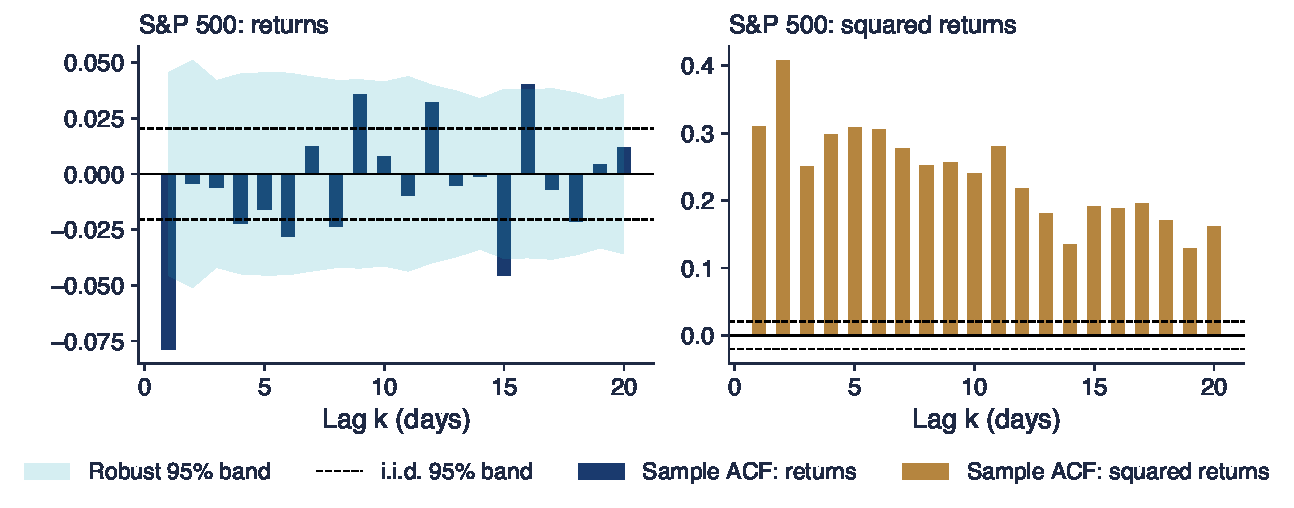
\includegraphics[width=0.96\textwidth,height=0.36\textheight,keepaspectratio]{ch7_sem_b1.pdf}
\end{center}
\vspace{-2mm}
\begin{itemize}
    \item $\hat\rho(1..5)$, randamente: $-0{,}079$; $-0{,}004$; $-0{,}006$; $-0{,}022$; $-0{,}016$; la pătrat: $0{,}311$; $0{,}408$; $0{,}250$; $0{,}298$; $0{,}308$; $T = 9\,240$
    \item Randamente: $Q_{LB}(10) = 90{,}8$ (p $<$\,0{,}001), $\tilde Q(10) = 18{,}8$ (p = 0{,}043); la pătrat: $Q_{LB}(10) = 8015$, $\tilde Q(10) = 189{,}4$ (ambele p $<$\,0{,}001)
    \item Interpretare: randamentele la pătrat resping RW1 (gruparea volatilității); testul robust respinge RW3 doar la limită, din cauza unui $\hat\rho(1)$ negativ mic: o revenire slabă, de scurtă durată
\end{itemize}\sfmquantlet{Ch_07}{SFM_ch7_seminar}
\end{frame}

\begin{frame}{B2: BET, Bitcoin și două acțiuni BVB [Propus]}
\itemsize{\footnotesize}
\begin{itemize}
\item \textbf{Întrebarea}: pentru care dintre BET, Bitcoin, Banca Transilvania și OMV Petrom se schimbă verdictul privind autocorelația între testul clasic și cel robust? Model: B1.
\item \textbf{Date}: BET din 1997, Bitcoin din 2014, TLV și SNP din 2010 (TLV fără 30--31 mai 2016), randamente logaritmice zilnice în \%
\item \textbf{Cerințe}
\begin{enumerate}
    \item Calculați $\hat\rho(1)$, $Q_{LB}(10)$ și $\tilde Q(10)$ cu p-valori pentru fiecare serie.
    \item Calculați statistica $z$ a testului runs și p-valoarea ei pentru fiecare serie.
    \item Marcați seriile pentru care testul clasic și cel robust nu sînt de acord la 5\%.
    \item Interpretare: de ce este BET diferit de celelalte trei?
\end{enumerate}
\item \textbf{Raportați}: un tabel și două fraze
\item Notebook: secțiunea B2
\end{itemize}
\end{frame}

\ifsolutions
\begin{frame}{B2: rezolvare [Propus]}
\itemsize{\footnotesize}
\begin{center}
\footnotesize
\begin{tabular}{lrrrrrrrr}
\toprule
& $T$ & $\hat\rho(1)$ & $Q_{LB}(10)$ & p & $\tilde Q(10)$ & p & runs $z$ & p \\
\midrule
BET & 7\,243 & ${0{,}156}$ & $198{,}3$ & $<$\,0{,}001 & $42{,}9$ & $<$\,0{,}001 & ${-7{,}75}$ & $<$\,0{,}001 \\
Bitcoin & 4\,384 & ${-0{,}022}$ & $20{,}2$ & 0{,}028 & $11{,}9$ & 0{,}294 & ${2{,}68}$ & 0{,}007 \\
TLV & 3\,788 & ${0{,}010}$ & $29{,}1$ & 0{,}001 & $13{,}2$ & 0{,}210 & ${-1{,}68}$ & 0{,}093 \\
SNP & 3\,815 & ${-0{,}015}$ & $20{,}7$ & 0{,}023 & $9{,}9$ & 0{,}446 & ${1{,}72}$ & 0{,}085 \\
\bottomrule
\end{tabular}
\end{center}
\begin{itemize}
    \item LB clasic respinge pentru toate patru; testul robust doar pentru BET: verdictul se schimbă pentru Bitcoin, TLV și SNP
    \item Runs: BET are mult prea puține secvențe ($z = -7{,}75$); Bitcoin are prea multe ($z = 2{,}68$): semnele alternează puțin mai des decît în cazul independenței
    \item Interpretare: BET este un indice de acțiuni tranzacționate inegal: prețurile de închidere vechi creează autocorelație pozitivă (thin trading); acțiunile individuale și Bitcoin nu o arată
\end{itemize}\sfmquantlet{Ch_07}{SFM_ch7_seminar}
\end{frame}
\fi

\begin{frame}{B3: rădăcini unitare în DAX [Rezolvat]}
\itemsize{\footnotesize}
\begin{itemize}
\item \textbf{Întrebarea}: care este ordinul de integrare al prețului logaritmic DAX și al randamentelor lui?
\item \textbf{Date}: închiderile DAX din 1990; prețul logaritmic și randamentele logaritmice zilnice
\item \textbf{Cerințe}
\begin{enumerate}
    \item Desenați prețul logaritmic cu o tendință liniară ajustată, precum și randamentele.
    \item Aplicați ADF (ordinul decalajelor ales prin AIC), PP și KPSS pe prețul logaritmic, cu constantă și tendință.
    \item Aplicați aceleași trei teste pe randamente, cu constantă.
    \item Interpretare: dovedește o rădăcină unitară în prețul DAX că DAX este eficient în formă slabă?
\end{enumerate}
\item \textbf{Raportați}: graficul, șase statistici cu p-valori și două fraze
\item Notebook: secțiunea B3
\end{itemize}
\end{frame}

\begin{frame}{B3: rezolvare [Rezolvat]}
\itemsize{\scriptsize}
\begin{center}
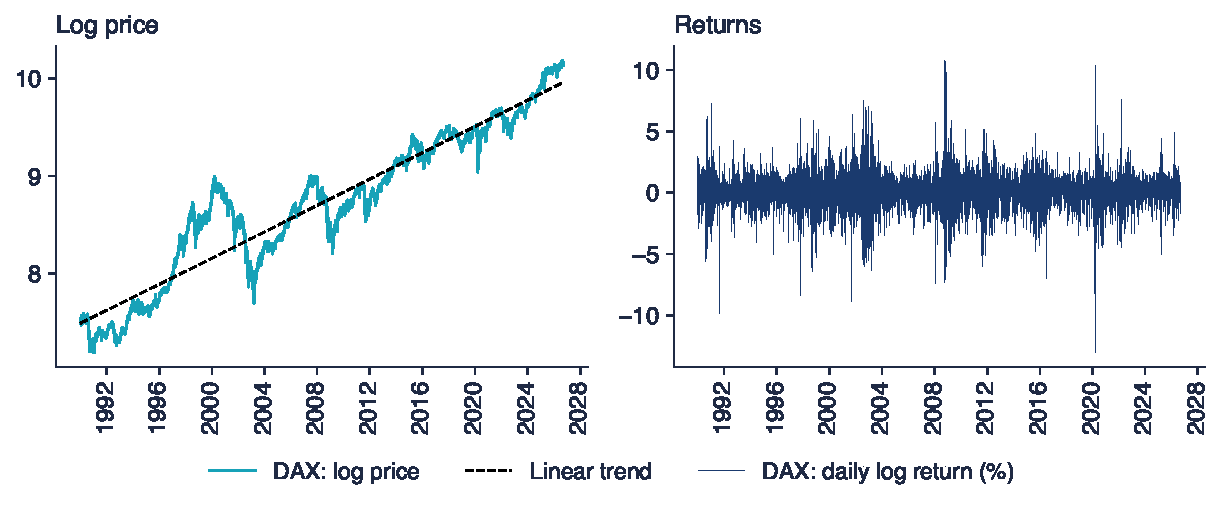
\includegraphics[width=0.96\textwidth,height=0.36\textheight,keepaspectratio]{ch7_sem_b3.pdf}
\end{center}
\vspace{-2mm}
\begin{center}
\scriptsize
\begin{tabular}{lrrr}
\toprule
& ADF & PP & KPSS \\
\midrule
preț logaritmic (tendință) & $-2{,}69$ (p = 0{,}239) & $-2{,}65$ (p = 0{,}260) & $0{,}94$ (p $<$\,0{,}01) \\
randamente (constantă) & $-23{,}30$ (p $<$\,0{,}001) & $-97{,}40$ (p $<$\,0{,}001) & $0{,}04$ (p $>$\,0{,}10) \\
\bottomrule
\end{tabular}
\end{center}
\begin{itemize}
    \item ADF a folosit 30 de decalaje pentru preț (AIC); PP și KPSS folosesc 38 de decalaje Bartlett; $T = 9\,288$
    \item Prețul: nicio respingere ADF sau PP, respingere KPSS: $I(1)$; randamentele: invers: $I(0)$
    \item Interpretare: nu; rădăcina unitară este necesară pentru un mers aleator, dar permite creșteri previzibile; eficiența se testează pe randamente (B1, B5)
\end{itemize}\sfmquantlet{Ch_07}{SFM_ch7_seminar}
\end{frame}

\begin{frame}{B4: BET, Bitcoin și TLV [Propus]}
\itemsize{\footnotesize}
\begin{itemize}
\item \textbf{Întrebarea}: sînt de acord cele trei teste de rădăcină unitară pentru BET, Bitcoin și Banca Transilvania? Model: B3.
\item \textbf{Date}: BET din 1997, Bitcoin din 2014, TLV din 2010 (fără 30--31 mai 2016)
\item \textbf{Cerințe}
\begin{enumerate}
    \item Aplicați ADF, PP și KPSS pe fiecare preț logaritmic (constantă și tendință) și pe fiecare serie de randamente (constantă).
    \item Clasificați fiecare serie ca $I(1)$, $I(0)$ sau neconcludentă.
    \item Pentru un caz neconcludent, propuneți o verificare care l-ar putea lămuri.
    \item Interpretare: ați tranzacționa pe baza acestei dovezi un preț TLV „care revine la medie”?
\end{enumerate}
\item \textbf{Raportați}: un tabel, trei clasificări și două fraze
\item Notebook: secțiunea B4
\end{itemize}
\end{frame}

\ifsolutions
\begin{frame}{B4: rezolvare [Propus]}
\itemsize{\footnotesize}
\begin{center}
\scriptsize
\begin{tabular}{lrrrrrr}
\toprule
& ADF preț (p) & PP preț (p) & KPSS preț (p) & ADF rand. & PP rand. & KPSS rand. (p) \\
\midrule
BET & ${-1{,}73}$ (0{,}736) & ${-1{,}54}$ (0{,}814) & $2{,}30$ ($<$\,0{,}01) & ${-13{,}65}$ & ${-74{,}47}$ & $0{,}12$ ($>$\,0{,}10) \\
Bitcoin & ${-1{,}48}$ (0{,}837) & ${-1{,}54}$ (0{,}817) & $1{,}81$ ($<$\,0{,}01) & ${-20{,}16}$ & ${-67{,}84}$ & $0{,}13$ ($>$\,0{,}10) \\
TLV & ${-3{,}46}$ (0{,}044) & ${-3{,}35}$ (0{,}058) & $0{,}57$ ($<$\,0{,}01) & ${-12{,}96}$ & ${-60{,}79}$ & $0{,}23$ ($>$\,0{,}10) \\
\bottomrule
\end{tabular}
\end{center}
\begin{itemize}
    \item BET și Bitcoin: preț logaritmic $I(1)$, randamente $I(0)$
    \item Prețul TLV: ADF respinge la 5\% (p = 0{,}044), PP nu (p = 0{,}058), KPSS respinge staționaritatea: neconcludent; verificare: testați o ruptură structurală sau împărțiți eșantionul
    \item Interpretare: nu; o p-valoare la limită, contrazisă de alte două teste, pentru una dintre multe serii testate, nu este un semnal de tranzacționare
\end{itemize}\sfmquantlet{Ch_07}{SFM_ch7_seminar}
\end{frame}
\fi

\begin{frame}{B5: rapoartele varianțelor pentru S\&P 500 [Rezolvat]}
\itemsize{\footnotesize}
\begin{itemize}
\item \textbf{Întrebarea}: revine S\&P 500 la medie pe orizonturi de 2--20 de zile, dacă ținem cont de gruparea volatilității?
\item \textbf{Date}: închiderile S\&P 500 din 1990, randamente logaritmice zilnice în \%
\item \textbf{Cerințe}
\begin{enumerate}
    \item Calculați VR($q$), $Z(q)$ și $Z^*(q)$ pentru $q = 2, 5, 10, 20$.
    \item Calculați statistica Chow--Denning și comparați-o cu valoarea ei critică de 5\%.
    \item Desenați VR($q$) pentru $q = 2, \dots, 40$ cu benzile de 95\% i.i.d.\ și robustă.
    \item Interpretare: este revenirea la medie suficient de mare pentru a conta pentru un investitor?
\end{enumerate}
\item \textbf{Raportați}: un tabel cu douăsprezece cifre, o statistică, graficul și două fraze
\item Notebook: secțiunea B5
\end{itemize}
\end{frame}

\begin{frame}{B5: rezolvare [Rezolvat]}
\itemsize{\scriptsize}
\begin{center}
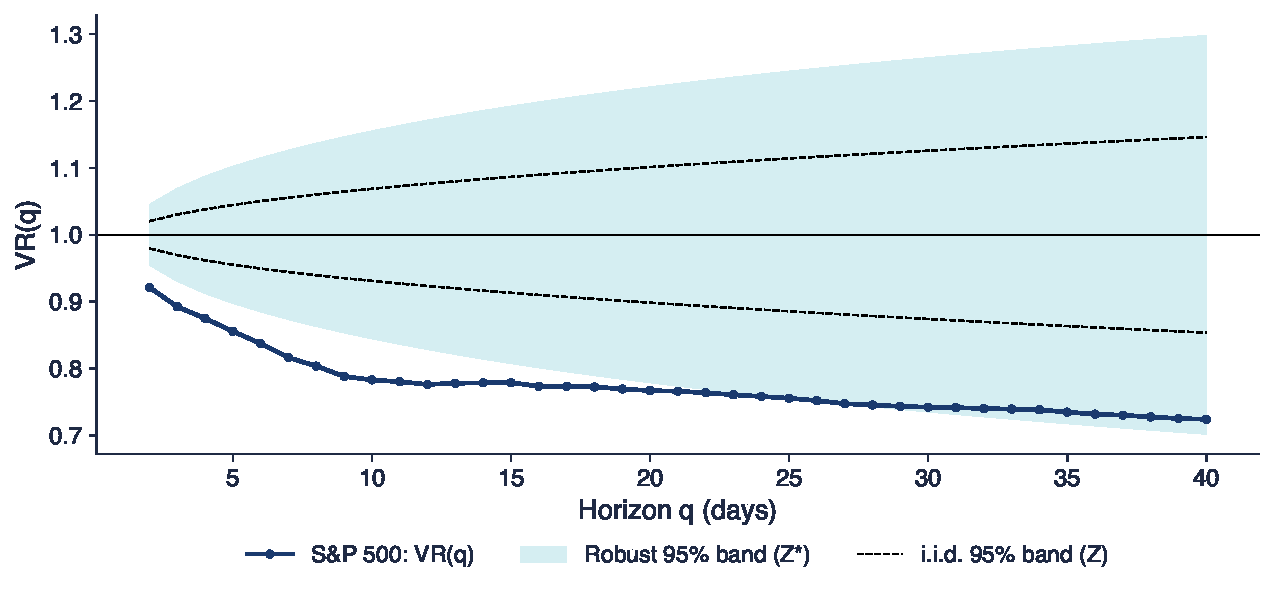
\includegraphics[width=0.96\textwidth,height=0.32\textheight,keepaspectratio]{ch7_sem_b5.pdf}
\end{center}
\vspace{-2mm}
\begin{center}
\scriptsize
\begin{tabular}{lrrrr}
\toprule
& $q = 2$ & $q = 5$ & $q = 10$ & $q = 20$ \\
\midrule
VR($q$) & $0{,}922$ & $0{,}856$ & $0{,}783$ & $0{,}767$ \\
$Z(q)$ & ${-7{,}54}$ & ${-6{,}33}$ & ${-6{,}17}$ & ${-4{,}50}$ \\
$Z^*(q)$ & ${-3{,}37}$ & ${-2{,}76}$ & ${-2{,}73}$ & ${-2{,}06}$ \\
\bottomrule
\end{tabular}
\end{center}
\begin{itemize}
    \item $T = 9\,240$; Chow--Denning: $\max|Z^*| = 3{,}37 > 2{,}49$ (p = 0{,}003): respingem mersul aleator
    \item $Z(2)$ este de circa 2{,}2 ori $Z^*(2)$: ignorarea grupării volatilității exagerează dovezile
    \item Interpretare: semnificativă, dar mică: varianța săptămînală este circa 86\% din cinci varianțe zilnice; după costurile de tranzacționare, cu greu un profit
\end{itemize}\sfmquantlet{Ch_07}{SFM_ch7_seminar}
\end{frame}

\begin{frame}{B6: cinci piețe emergente [Propus]}
\itemsize{\footnotesize}
\begin{itemize}
\item \textbf{Întrebarea}: care dintre WIG20, BUX, PX, BET și BIST 100 se abate de la un mers aleator în ultimii zece ani? Model: B5.
\item \textbf{Date}: randamente logaritmice zilnice de la 19 septembrie 2016 pînă la 18 septembrie 2026
\item \textbf{Cerințe}
\begin{enumerate}
    \item Calculați VR(5), $Z^*(5)$ și p-valoarea lui pentru fiecare piață.
    \item Calculați p-valoarea Chow--Denning ($q = 2, 5, 10, 20$) și testul VR automat cu p-valoarea wild bootstrap.
    \item Calculați valoarea critică Šidák pentru cinci piețe testate împreună la 5\%.
    \item Interpretare: ce piețe ați numi ineficiente, după ce țineți cont de testarea a cinci piețe?
\end{enumerate}
\item \textbf{Raportați}: un tabel, o valoare critică și două fraze
\item Notebook: secțiunea B6
\end{itemize}
\end{frame}

\ifsolutions
\begin{frame}{B6: rezolvare [Propus]}
\itemsize{\footnotesize}
\begin{center}
\footnotesize
\begin{tabular}{lrrrrrrr}
\toprule
& $T$ & VR(5) & $Z^*(5)$ & p & CD p & VR automat & p (bootstrap) \\
\midrule
WIG20 & 2\,498 & $0{,}979$ & ${-0{,}27}$ & 0{,}789 & 0{,}938 & ${-1{,}09}$ & 0{,}342 \\
BUX & 2\,492 & $1{,}033$ & ${0{,}33}$ & 0{,}739 & 0{,}995 & ${0{,}01}$ & 0{,}992 \\
PX & 2\,504 & $1{,}206$ & ${2{,}08}$ & 0{,}038 & 0{,}142 & ${2{,}56}$ & 0{,}104 \\
BET & 2\,492 & $1{,}200$ & ${2{,}03}$ & 0{,}042 & 0{,}159 & ${3{,}76}$ & 0{,}034 \\
BIST 100 & 2\,507 & $1{,}086$ & ${1{,}34}$ & 0{,}180 & 0{,}549 & ${0{,}04}$ & 0{,}868 \\
\bottomrule
\end{tabular}
\end{center}
\begin{itemize}
    \item Šidák: fiecare test la $1 - 0{,}95^{1/5} = 1{,}02\%$, valoarea critică $2{,}57$; cu cinci teste independente la 5\%, șansa a cel puțin unei respingeri false este 22{,}6\%
    \item PX și BET: $Z^*(5)$ puțin peste 1,96, sub $2{,}57$; Chow--Denning nu respinge; doar VR automat respinge pentru BET
    \item Interpretare: nicio piață nu este clar ineficientă; BET arată un momentum slab, care depinde de test
\end{itemize}\sfmquantlet{Ch_07}{SFM_ch7_seminar}
\end{frame}
\fi


%=============================================================================
\section{Partea C: întrebări deschise și critica unui răspuns AI}
%=============================================================================

\begin{frame}{C1: a devenit BET mai eficient? [Propus]}
\itemsize{\footnotesize}
\begin{itemize}
\item \textbf{Întrebarea}: cum a evoluat previzibilitatea BET din 1997 pînă azi, inclusiv în jurul trecerii la Secondary Emerging de către FTSE Russell în septembrie 2020?
\item \textbf{Date}: randamentele logaritmice zilnice BET din 1997; modele: B1, B5
\item \textbf{Cerințe}
\begin{enumerate}
    \item Calculați VR(5) și $Z^*(5)$ pe ferestre mobile de 500 de zile, una la fiecare 21 de zile, și ponderea ferestrelor cu $|Z^*(5)| > 1{,}96$ în primii și în ultimii cinci ani.
    \item Calculați $\hat\rho(1)$, VR(5), $Z^*(5)$ și p-valoarea Chow--Denning în 1997--2006, 2007--2016 și 2017--2026.
    \item Comparați VR(5) în cei cinci ani dinainte și de după 21 septembrie 2020.
    \item Enumerați ce altceva s-a schimbat pe piața românească în același timp.
    \item Interpretare: cum ați separa aceste schimbări de efectul trecerii la noul statut?
\end{enumerate}
\item \textbf{Raportați}: un tabel, un grafic și un plan de proiect
\item Notebook: secțiunea C1
\end{itemize}
\end{frame}

\ifsolutions
\begin{frame}{C1: analiză de referință [Propus]}
\itemsize{\footnotesize}
\begin{center}
\footnotesize
\begin{tabular}{lrrrrr}
\toprule
Perioada & $T$ & $\hat\rho(1)$ & VR(5) & $Z^*(5)$ & CD p \\
\midrule
1997--2006 & 2306 & $0{,}270$ & $1{,}50$ & $6{,}15$ & $<$\,0{,}001 \\
2007--2016 & 2516 & $0{,}066$ & $1{,}08$ & $0{,}82$ & 0{,}262 \\
2017--2026 & 2421 & $0{,}064$ & $1{,}20$ & $2{,}04$ & 0{,}154 \\
\bottomrule
\end{tabular}
\end{center}
\begin{itemize}
    \item Ferestre mobile care resping la 5\%: 89\% în primii cinci ani, 15\% în ultimii cinci ani
    \item Cinci ani înainte și după: VR(5) $1{,}12$ ($Z^* = 0{,}80$) și $1{,}18$ ($Z^* = 1{,}78$); diferența $z = 0{,}34$: nicio dovadă
    \item Factori care se suprapun: COVID-19 (2020), listarea Hidroelectrica (2023), volumele, componența indicelui; variante: același test pe acțiunile BVB, WIG20 și BUX drept comparație
\end{itemize}\sfmquantlet{Ch_07}{SFM_ch7_seminar}
\end{frame}
\fi

\begin{frame}{C2: verificați un răspuns AI [Propus]}
\itemsize{\scriptsize}
\begin{itemize}
    \item Un student a cerut unui asistent AI să spună dacă DAX (zilnic, din 1990) este eficient în formă slabă. Răspunsul:
    \item \aiprompt{(a) ADF pe prețul logaritmic DAX dă tau = -2{,}69, p = 0{,}24: rădăcina unitară nu este respinsă, deci DAX este eficient în formă slabă.}
    \item \aiprompt{(b) Ljung-Box Q(10) = 21{,}83, p = 0{,}016: randamentele DAX sînt previzibile, deci DAX nu este eficient.}
    \item \aiprompt{(c) Pentru randamentele la pătrat Q(10) = 3747: randamentele DAX nu sînt un martingal.}
    \item \aiprompt{(d) VR(10) = 0{,}93 < 1 arată autocorelație pozitivă (momentum) în DAX.}
    \item \aiprompt{(e) Pentru RW1, VR(q) = 1 la orice orizont, iar varianța randamentelor pe q zile este de q ori varianța zilnică.}
    \item Cerințe
    \begin{itemize}
        \item 1. Pentru fiecare afirmație spuneți dacă este corectă; dacă nu, dați afirmația corectă și, unde se poate, cifra corectă din notebook (secțiunea C2).
        \item 2. Raportați: o listă de cinci verdicte, fiecare cu un rînd de justificare.
    \end{itemize}
\end{itemize}
\end{frame}

\ifsolutions
\begin{frame}{C2: rezolvare [Propus]}
\itemsize{\footnotesize}
\begin{itemize}
    \item (a) Greșit: rădăcina unitară este necesară, nu suficientă; prețurile $I(1)$ pot avea creșteri previzibile; testați randamentele
    \item (b) Greșit: $Q_{LB}$ presupune randamente i.i.d.; $\tilde Q(10)$ robust $= 8{,}59$ (p = 0{,}571) nu respinge
    \item (c) Greșit: randamentele la pătrat corelate înseamnă gruparea volatilității; resping RW1, nu martingalul ($\tilde Q$ robust al pătratelor: $334{,}3$, tot doar RW1)
    \item (d) Greșit: VR $< 1$ înseamnă autocorelație negativă (revenire la medie), iar $Z^*(10) = -1{,}21$ nu este semnificativ ($Z(10) = -1{,}95$)
    \item (e) Corect: $\mathrm{Var}(r_t(q)) = q\sigma^2$ pentru RW1 (de fapt și pentru RW3)
\end{itemize}\sfmquantlet{Ch_07}{SFM_ch7_seminar}
\end{frame}
\fi


%=============================================================================
\section{Încheiere}
%=============================================================================

\begin{frame}{Idei de reținut}
\itemsize{\small}
\begin{itemize}
    \item O rădăcină unitară în prețuri este punctul de plecare, nu răspunsul: eficiența privește randamentele
    \item Testați martingalul cu statistici robuste ($\tilde Q$, $Z^*$): testele clasice confundă gruparea volatilității cu previzibilitatea
    \item VR $> 1$: momentum; VR $< 1$: revenire la medie; S\&P 500 revine ușor, vechiul BET urma tendința
    \item Multe orizonturi sau multe piețe: folosiți Chow--Denning sau o corecție Šidák
    \item Un răspuns AI este o ciornă: verificați ipoteza nulă a fiecărui test, semnul lui VR $- 1$ și versiunea robustă
\end{itemize}
\end{frame}

\begin{frame}{După seminar}
\itemsize{\small}
\begin{itemize}
    \item Cursul 7 dezvoltă fiecare temă de azi: eficiența, mersul aleator, testele ACF, rădăcinile unitare, rapoartele varianțelor, piețele adaptive
    \item Încercați cerințele [Propus] în notebook; rezolvările se discută la seminar
    \item C1 poate deveni un proiect de echipă: acțiunile din BET, WIG20 și BUX drept comparație, un bootstrap pe blocuri al diferenței
    \item Lectură: \refFHH, cap.~11; exerciții în \refBHL, cap.~11; \refCLM, cap.~2
\end{itemize}
\end{frame}


%=============================================================================
\section{Bibliografie}
%=============================================================================

\begin{frame}{Bibliografie}
\itemsize{\tiny}
\begin{itemize}
    \item Borak, S., Härdle, W.K., López-Cabrera, B. (2013). \href{https://doi.org/10.1007/978-3-642-33929-5}{\textit{Statistics of Financial Markets: Exercises and Solutions}}, 2nd ed. Springer.
    \item Box, G.E.P., Pierce, D.A. (1970). \href{https://doi.org/10.1080/01621459.1970.10481180}{Distribution of residual autocorrelations in autoregressive-integrated moving average time series models}. \textit{Journal of the American Statistical Association}, 65(332), 1509--1526.
    \item Campbell, J.Y., Lo, A.W., MacKinlay, A.C. (1997). \href{https://doi.org/10.1515/9781400830213}{\textit{The Econometrics of Financial Markets}}. Princeton University Press.
    \item Choi, I. (1999). \href{https://doi.org/10.1002/(SICI)1099-1255(199905/06)14:3<293::AID-JAE503>3.0.CO;2-5}{Testing the random walk hypothesis for real exchange rates}. \textit{Journal of Applied Econometrics}, 14(3), 293--308.
    \item Chow, K.V., Denning, K.C. (1993). \href{https://doi.org/10.1016/0304-4076(93)90051-6}{A simple multiple variance ratio test}. \textit{Journal of Econometrics}, 58(3), 385--401.
    \item Dickey, D.A., Fuller, W.A. (1979). \href{https://doi.org/10.1080/01621459.1979.10482531}{Distribution of the estimators for autoregressive time series with a unit root}. \textit{Journal of the American Statistical Association}, 74(366), 427--431.
    \item Escanciano, J.C., Lobato, I.N. (2009). \href{https://doi.org/10.1016/j.jeconom.2009.03.001}{An automatic Portmanteau test for serial correlation}. \textit{Journal of Econometrics}, 151(2), 140--149.
    \item Fama, E.F. (1970). \href{https://doi.org/10.1111/j.1540-6261.1970.tb00518.x}{Efficient capital markets: a review of theory and empirical work}. \textit{Journal of Finance}, 25(2), 383--417.
    \item Franke, J., Härdle, W.K., Hafner, C.M. (2019). \href{https://doi.org/10.1007/978-3-030-13751-9}{\textit{Statistics of Financial Markets: An Introduction}}, 5th ed. Springer.
    \item Kim, J.H. (2009). \href{https://doi.org/10.1016/j.frl.2009.04.003}{Automatic variance ratio test under conditional heteroskedasticity}. \textit{Finance Research Letters}, 6(3), 179--185.
    \item Kwiatkowski, D., Phillips, P.C.B., Schmidt, P., Shin, Y. (1992). \href{https://doi.org/10.1016/0304-4076(92)90104-Y}{Testing the null hypothesis of stationarity against the alternative of a unit root}. \textit{Journal of Econometrics}, 54(1--3), 159--178.
    \item Ljung, G.M., Box, G.E.P. (1978). \href{https://doi.org/10.1093/biomet/65.2.297}{On a measure of lack of fit in time series models}. \textit{Biometrika}, 65(2), 297--303.
    \item Lo, A.W., MacKinlay, A.C. (1988). \href{https://doi.org/10.1093/rfs/1.1.41}{Stock market prices do not follow random walks: evidence from a simple specification test}. \textit{Review of Financial Studies}, 1(1), 41--66.
    \item MacKinnon, J.G. (1996). \href{https://doi.org/10.1002/(SICI)1099-1255(199611)11:6<601::AID-JAE417>3.0.CO;2-T}{Numerical distribution functions for unit root and cointegration tests}. \textit{Journal of Applied Econometrics}, 11(6), 601--618.
    \item Phillips, P.C.B., Perron, P. (1988). \href{https://doi.org/10.1093/biomet/75.2.335}{Testing for a unit root in time series regression}. \textit{Biometrika}, 75(2), 335--346.
    \item Said, S.E., Dickey, D.A. (1984). \href{https://doi.org/10.1093/biomet/71.3.599}{Testing for unit roots in autoregressive-moving average models of unknown order}. \textit{Biometrika}, 71(3), 599--607.
    \item Wald, A., Wolfowitz, J. (1940). \href{https://doi.org/10.1214/aoms/1177731909}{On a test whether two samples are from the same population}. \textit{Annals of Mathematical Statistics}, 11(2), 147--162.
\end{itemize}
\end{frame}

\end{document}
